% \documentclass{article}
% \documentclass[final, 12pt, a4paper, twoside, english, indent]{itthesis}

\documentclass[12pt, twoside, a4paper, english]{./Help/Templates/MIT/mitthesis}
\usepackage{./Help/Templates/MIT/lgrind}
\pagestyle{plain}
 
\usepackage[pdftex, pdftitle={}, pdfauthor={Dmitry Myadzelets}, bookmarks=true,
% colorlinks=true, linkcolor=black
]{hyperref}

% Mathematical symbols
\usepackage{amsfonts, amssymb, amsmath, amsthm}

% Figures
\usepackage{tikz} 
\usetikzlibrary{decorations.pathreplacing}
\usetikzlibrary{arrows,positioning,automata,shadows,fit,shapes}

% Folder all the pictures are located
\graphicspath{{figures/}}

% For color backgound of figures 
% \usepackage{mdframed}
% \let\originalfigure=\figure
% \let\endoriginalfigure=\endfigure
% \renewenvironment{figure}[1][]{
%   \begin{originalfigure}[#1]
%     \begin{mdframed}[linecolor=black!0,backgroundcolor=blue!5]
% }{
%     \end{mdframed}
%   \end{originalfigure} 
% } 

% URL in bibliography 
\usepackage{url} 

% Algorithms 
\usepackage{algpseudocode}
\usepackage{float}
\newfloat{alg}{t}{lop}
\floatname{alg}{Algorithm}

% Logarithmic plots in the simulation 
\usepackage{pgfplots}


\begin{document}

\include{cover}
% Some departments (e.g. 5) require an additional signature page.  See
% signature.tex for more information and uncomment the following line if
% applicable.
% \include{signature}
\pagestyle{plain}
\include{contents}

\chapter*{Introduction}
\addcontentsline{toc}{chapter}{Introduction}


% \section{Introducton to Introduction}

Modern society is characterized by the growing demand for the use of automated
systems in the everyday life, and these systems require software engineering
with constantly increasing complexity. Industrial automation software
engineering has traditionally been a field with the most strict requirements
and highest standards applied. However, it is still a common practice for an
automation software design to consist of writing a ladder logic for programmable
logic controller (PLC) with partially and ambiguously determined specifications,
without clearly defined software architecture, and no formal verification of the
system.
Reflecting the importance of the software and a growing ratio of the software
cost to the costs of machinery, engineers and researches put a lot of effort
toward facilitating the development and maintenance of software, increasing its
performance and reliability while decreasing the cost of its life cycle. One of
the major established trends is use of standardised component solutions for
industrial automation systems aiming at portability, reusability,
interoperability and reconfiguration of applications. Another tendency is
the growing number of formal methods - mathematical approaches supporting
decisions making process during systems design and operations.

\section*{Design Process of Industrial Systems}

According to the standard ISO/IEC 12207 \cite{_iso/iec_12207_2008} the
industrial software development process (life cycle process) can be structured
into six stages: requirements specification, software design, implementation and
integration, testing, deployment and maintenance. Starting from the
implementation the stages mainly depend on a particular vendor of hardware
and a dedicated software - supervisory control acquisition system (SCADA).
There are hundreds of major producers of automation hardware and software, but
the variety of ways the developers can write programs is limited by the standards,
such as {IEC 61131}, making them less error prone and more reusable. In other
words, this sequence of stages is quite mature. 

The stage of requirements specification consists of analyzing, documenting and
validating the needs and conditions for technological process, as well as rules,
constrains and policies for the plant hardware. The most known standard used at
this stage is the Unified Modeling Language (UML), developed by the Object
Management Group (OMG) Technology Standards Consortium. This standard
facilitates also the next stage, software design, with a Model-Driven
Architecture (MDA) approach. The industrial software design stage adopts
numerous methods, such as component based approach, object-oriented and
aspect-oriented programming, and software product line, etc (see
\cite{vyatkin_software_2013} for an extensive survey of the state of the art for
software engineering methods in industrial automation).

\section*{Problems Statement}

The major drawback of the aforementioned industrial software
development process is that it is mainly designed for humans, whereas the
reliability and other important properties of systems in large part depend on
machine-oriented formal verification methods. Formal methods apply
mathematically-based techniques to the development of systems, from the
specification level to the implementation level. These methods proved
to be effective, especially for safety critical systems, but due to their
mathematical nature and lack of the supporting tools the use of formal methods
in industrial practice is not common yet. The problem is that mathematical
notation requires to have additional knowledge on the part of the development
engineers, creating a psychological barrier for them, and also that the 'de
facto' development process does not incorporate a formal representation.

A way to overcome the above problem is to mix formal techniques with
``standard-based'' approaches/tools which are already adopted in industry. If
a non formal (or semi-formal) systems representation has the ability to be
translated into a completely formal form, then mathematical techniques can be
applied. Examples of such approaches are \cite{dong_model_2001}, where authors
extend UML representation with a ``collaboration diagram'' and translate it to
extended hierarchical automata, \cite{secchi_use_2007} which formalizes UML
into Dirac structures, and \cite{zhou_semantic_2012} where the authors
translate Simulink diagrams into input/output extended finite automata.

Even though the translation into a mathematical representation gives the
opportunity to apply formal techniques, the requirements for the system's
properties should again be expressed in a formal way by engineers, which
raises the above mentioned problems. Thus, despite of the fact that some
successful reports can be found in literature, progress along these lines seems
minimal
% , andapplicable only with numerous constrains both for the methods and the tools
. 

Another solution to overcome the problem is the development of new approaches
which incorporate advantages of both methodologies, the one suitable for humans,
and the other using formal techniques. Nowadays, when the growing complexity of
automated systems imposes requirements which can be met only by formal methods,
the relevant response may be the creation of modeling techniques when the models
already encapsulate their formal representations. Thus, the underlining
mathematical nature would be ``hidden'' from engineers, and verification of
important properties can be performed automatically. An example of such approach
is presented in \cite{sartini_architectures_2010} where the authors propose
a library of general UML blocks where each block is corresponded to a predefined
automaton. The simple blocks can be used then to construct more complex
entities while their formal representation can be achieved automatically by
composition of the predefined automata.

The necessity of composition of modules formal representations for the sake of
verification of some important properties gives rise to another problem, which
is inseparable from the formal methods, - the problem of so-called \emph{state
explosion}. This problem can be solved by development of mathematical
techniques which efficiently exploit the modular nature of the systems such
that the corresponding computational burden remains at an acceptable level.

As soon as the quantity and quality of mathematical methods and their
implementations is sufficient for the current complexity of automated systems,
and these methods can be encapsulated into integrated development tools as a
first-class citizen, seamlessly providing the power of formal approaches through
the easy-to-understand visual modeling process, the development process of
automated systems will move to the next stage of its evolution.

\section*{Contribution}

This work aims to facilitate the process of industrial automated systems
development applying formal methods to ensure the reliability of systems. From
many existing problems, for this work has been chosen the problem of
verification of system's design in terms of diagnosability. Diagnosability
problem answers the question: either the given system is ready for fault
diagnosis or not. According to the IEC vocabulary \cite{iec_vocabulary} the
\emph{fault diagnosis} are ``actions taken for fault recognition, fault
localization and cause identification'', and a \emph{fault} is ``the state of an
item characterized by inability to perform a required function''.

To achieve the goals, this work exploits Discrete Event Systems theory
\cite{cassandras_introduction_2010} and its automata framework. The theory of
automata is chosen due to its relative simplicity. Indeed, it has just two basic
entities (state and event) and intuitively intelligible graphical
representation. Taking apart a language theory, which is necessary for
research, the automata framework does not require much additional
mathematical knowledge for automation engineers. This makes it the first
candidate as a formal mathematical tool for future general purpose integrated
development environments (IDE) in automation industry.

The main contributions are following:
\begin{itemize}
  \item A new formulation of distributed diagnosability problem. This 
  formulation is then used to enforce the desired property of the system,
  rather then just verifying it. This approach tackles the state explosion problem
  which arises when the automata framework is applied for complex discrete event
  systems.
  \item Presented new structural patterns, in terms of automata
  framework. These patterns are aimed to decrease computation burden while
  applying verification algorithms.
  \item Created algorithms for verification of diagnosability property in the
  context of the new distributed diagnosability problem.
  \item Extended the approach of \emph{GeneralizedDevice}, recently
  developed in the University of Bologna \cite{faldella_hierarchical_2008},
  \cite{sartini_architectures_2010}. This work extends it towards formalization
  of failures representation in order to apply the developed algorithms. It
  allows the embedding of a formal approach into a higher level of the
  systems' representation of ``standard'' modular design process, similar to one
  exploiting UML design tools.
  \item To validate the concepts developed during the research, a software tool
  was created. This tool exploits web-technologies in order to provide zero-time
  access to it, the possibility for easy modifications in order to solve other
  formal problems, and opportunities for further enhancement by community.
\end{itemize}


\section*{Organization}

Chapter \ref{chap:problem_description} gives an overview of the problem of
fault diagnosis in a real example of an industrial automation plant. It
provides a short description of the technological process with a couple of
illustrative failures. The types of failures are discussed, and how particular
system's failures can be determined, evaluated and treated. 

Chapter \ref{chap:framework} describes the UML based modeling framework, and how 
the framework specifies hardware modules with automata. Then the
formal framework for discrete event systems is briefly presented, different
definitions of diagnosability are explained, and the general idea of new notion
of virtual modular diagnosability is given.

Chapter \ref{chap:theory} presents the new type of diagnosability -
virtual modular diagnosability, in details. It is firstly explained with a
simple example of a system consisting of two modules, then a general form of
the approach is described. At the end of the chapter algorithms for verification
of the virtual modular diagnosability are described.

Chapter \ref{chap:simulation} introduces a new tool for modeling and simulation
with automata. An application of the tool to the example of the real system
presented in the Chapter \ref{chap:problem_description} is shown.

The conclusions for the work are given at the end. 

% \emph{Formal methods aim to apply mathematically-based techniques to the
% development of computer-based systems, especially at the specification level,
% but also down to the implementation level. This aids early detection and
% avoidance of errors through increased understanding. It is also beneficial for
% more rigorous testing coverage. This talk presents the use of formal methods on
% a real project. The Z notation has been used to specify a large-scale high
% integrity system to aid in air traffic control. The system has been implemented
% directly from the Z specification using SPARK Ada, an annotated subset of the
% Ada programming language that includes assertions and tool support for proofs.
% The Z specification has been used to direct the testing of the software through
% additional test design documents using tables and fragments of Z. In addition,
% Mathematica has been used as a test oracle for algorithmic aspects of the
% system. In summary, formal methods can be used successfully in all phases of the
% lifecycle for a large software project with suitably trained engineers, despite
% limited tool support.}
% 
% \emph{Formal methods have been advocated as a means of increasing the
% reliability of systems, especially those which are safety or business critical,
% but the industrial uptake of such methods has been slow. This is due to the
% perceived difficulty of mathematical nature of these methods, the lack of tool
% support, and the lack of precedents where formal methods has been proved to be
% effective. It is even more difficult to develop automatic specification and
% verification tools due to limitations like state explosion, undecidability,
% etc.}


\chapter{Failure Diagnosis for Industrial Automation Plant}
\label{chap:problem_description}

This chapter uses an example of industrial automation plant to present the
problem of fault diagnosis. After a short description of the technological
process it shows two cases of failures. Then the types of failures are
discussed, and what approaches are adopted in industrial and academic
practices.

\section{Case Study of the Automated System}

An instance of the real automated systems is exploited to explain the problem of
failure diagnosis. It is a dust cleaner at an aluminium smelter. The Figure
\ref{fig:pi_diagram} depicts a simplified Piping and Instrumentation (P\&I) of
the system.

\subsection{Technological process}

\begin{figure}
  \includegraphics[width=\textwidth, keepaspectratio, angle=0] 
  {process-and-instrument-drawing.pdf}
  \caption{Piping and Instrumentation (P\&I) diagram of a dust cleaning system
  at an aluminium smelter}
  \label{fig:pi_diagram}
\end{figure}

For the given system two flows can be distinguished in the technological
process.
The first is the air flow which is blown trough a series of containers (the
figure depicts only one container, for simplicity). Each container is equipped with an
electrostatic filter.
The second flow is the flow of a dust. The dust comes with the air, sticks to
the filter, and then falls down to the bunker. Periodically the dust collected
in the bunker is transported out to a silos.

For the proper dust cleaning, the following parameters of the air flow have to
be maintained: a constant difference between the output and the input
pressures of the container, and a temperature at the input of the container. The
pressure is regulated by the valve $V$--2, which changes the area flow before
the pump $P$--1.
The temperature is regulated by the valve $V$--1 which changes the area flow 
of a preheated air. The air at the entrance of the filter is, thus, a mix of
the the polluted air and the preheated air. The temperature of this mix should
be higher then a certain point such that no condensation inside of the container
is guaranteed.

When the amount of the dust collected at the bottom of the container reaches a
necessary volume, i.e. it reaches a certain level, the dust is removed by the
screw conveyer. The gate valve $V$--3 is normally opened, since the screw of the
conveyer blocks the flow of the dust automatically when it is stopped. The belt
conveyer, in its turn, starts to work whenever one of the screw conveyers
starts. It delivers the dust to a dust bucket.

The dust bucket collects the dust until a volume of the dust is enough to pass
it down, to a pneumatic container. Then the gate valve $V$--4 opens and the
dust fills the container. Then the gate valve $V$--4 closes and the gate valve
$V$--5 opens allowing the compressed air to come to the container. Under a high
pressure the mix of the dust and the air is transported to a silos.

Periodically, in order to prevent sticking of the dust to the walls of the
container with electrostatic filters, the vibration machine $M$--1 has to be
switch on for a few seconds.


\subsection{Control System}

% Description of the control system (Siemens, etc.) (picture of PLC, Control
% station and etc, showing distributed nature of the system)

The control system consists of a PLC (Siemens Simatic S7--300
\cite{simatic_s7_300}), remote acquisition modules and an operator station
(with Siemens WinCC software) connected via industrial network. The PLC is
mounted near the field equipment, the operator station is located a few hundreds
meters away. 

The control systems has a few control cycles. Starting to the bottom-up
direction, the first cycle controls emptiness of the dust bucket with two level
sensors, $LT3$ and $LT4$. When a level of the dust reaches the high level
sensor $LT3$, the system starts to empty the bucket with the pneumatic container
until a level of the dust reaches the low level sensor $LT4$. The weight meter
$WT1$ is used to collect the statistic, and its measurements can be also used to
evaluate the amount of the dust in the container. The air flow meter $FT1$ is
aimed to collect statistical data too.

The second control cycle regulates the filling of the dust bucket. When the
dust level in the bucket is lower then the high level sensor $LT3$, and there is
an enabling signal from the upper (with respect to the material flow) control
cycle, it turns on the belt conveyer and enables a signal to one of the upper
control cycles (each container with its filter has its own control cycle).
Either the level of the dust in the bucket reaches the high level sensor $LT3$
or there is no any enabling signals from the upper control cycles, then the belt
conveyer stops.

The third control cycle regulates the level of the dust in the container
with the filter (the cycle is the same for each container). When the dust level
reaches the high level sensor $LT1$, it gives enabling signal to the below
control cycle of the belt conveyer and waits for enabling signal from it. After
receiving the enabling signal, the control cycle switches on the screw conveyer.
Ether the container becomes empty, i.e. the dust level decreases below the low
level sensor $LT2$, or the control cycle receives disabling signal from the
below control cycle, then it switches the screw conveyer off.

The forth control cycle regulates an order the containers with the filters
should be emptied. If more than one container is ready, i.e. the level of the
dust reached its high level sensor, then the first container has a priority,
since the speed it is filled with dust is faster. Then the second
container is emptied and so forth.

The fifth control cycle switches on vibration machines periodically, but only
when the container is being emptied.

All the actuators of the system can be in three states: disabled for operation,
manual control or automatic control. A signal corresponding to
the current state of each actuator is received by the PLC.


\subsection{Failures of the system}

The system can be affected by different types of failures, which may be
classified into the following categories with respect to likelihood the failure
occurs (the first type has the highers rate of occurrence):

\begin{itemize}
  \item Failures of the technological process
  \item Failures of mechanical devices
  \item Failures of electric and electronic components of the control system
\end{itemize}

Moreover, the failures can be external or internal with respect to the given
system. Yet another type of failure is one when malfunction of the system's
behavior is caused by an inconsistent human (operator) intrusion; it has left
outside of the scope. Some of the possible failures are described further,
according to the above classification.

\subsubsection{Failures of the technological process}

The technological failures might be caused by deviation of properties of the
materials involved in the process. Particularly in this system, a deviation of
the dust's or air's humidity can result in that the dust sticks to the filter,
to the walls of the container and to pipes, and obstructs the flow of the material.
Whereas the temperature of the air (low value of which is the main reason for
the condensation) is controlled, the humidity is not measured.

The air, coming to the pneumatic container has neither a temperature nor
humidity control. Additionally, the rise of the material humidity may happen due
to a leak of rainwater from the building's roof, and etc.

In general, technological failures are hard to predict, since there is
usually a little of statistical information for the particular process, if any. 

\subsubsection{Failures of the mechanical devices}

Malfunction of field mechanical devices, probably, is the most frequent reason
the automatic systems fail. Firstly, the field devices are exposed to hard
environmental conditions, such as temperature, vibration, humidity,
electromagnetic field, mechanical impact and etc. Secondly, they are normally
complex devices, composed of many other components, and thus the failure rate of
a complex device is higher then the highest failure rate of its modules.
A common solution adopted in industry is that all the actions performed under
each individual device, conditions under with the equipment is used, a time
duration it works, and etc. are journalized. These statistical information is
later used to plan and perform the maintaining and repairing.

The above presented system has following devices with mechanical parts and
parts which can be affected mechanically (e.g. by the flow of a material):
\begin{itemize}
  \item Butterfly valves $V$--1, $V$--2 and gate valves $V$--3, $V$--4, $V$--5.
  The weakest part of a valve is its actuator, which contains a plenty of
  moving components. Beside this, the valve's core is subject to abrasion. 
  \item The screw conveyer and the belt conveyer. These devices have a lot of
  moving components either, where the belt as the weakest part.  
  \item Electric motors $M$--1 -- 3 and pump $P$--1, which
  are subject to mechanical and electric damages.
  \item Weight meter $WT1$, with its fore tension meters which are subject to
  degradation.
  \item Fork level meters $LT1$ -- $4$. The forks are subject to abrasion.
  \item Pressure meters $PT1$, $PT2$. The drive mechanism of a pressure meter is
  the subject to stacking, dirt and oil clogging. 
\end{itemize}

All the above potential mechanical failures, the most of the listed above devices
contain electronic and electric components, which can have their one failures. 

\subsubsection{Failures of electric and electronic components}

Due to enormous amount electric and especially electronic components used in
modern manufacturing industry, it is quite impossible to make a classification
of all the failures which might occur, and it is seems useless to have such
information at the level of industrial automation, since a fault of a single
component most likely results in the failure of entire device it contains.
Instead, complex characteristics are used in order to be able to estimate 
possible faults. One of the well know parameters is the Mean time between
failures (MTBF). Another, relatively modern standard IEC 61511 also defines a
set of characteristics (MTBF and IEC 61511 are described briefly later).

\subsection{Examples of the systems' failures}

This work does not consider the question of faults prevention. The fact of a
fault occurrence has to be assumed, since the problem of the failure is not
only that it may lead the necessity to interrupt the technological process,
delay for delivery of spare parts and row materials. The major problem is that
one failure can sequentially cause other failures which may spread further
and so forth, with exponential growth, provoking a catastrophic impact at the
end.

As an example, the system presented in this chapter was subjected to 
some failures observed by the author of this work. These failures are
interesting from the point of view of their propagation.

In the first case the high level sensor $LT3$ failed while the system was at the
state of refilling the dust bucket. Since one of the conditions the control
system has to stops the filling is that the dust bucket is full, it was
delivering more and more material. The material overflowed the bucket in great
quantity, causing clogging of ventilation holes of the control system (which
later resulted in some spare parts change), and blocking entrance to the
building. The failure was spotted occasionally; elimination of its consequences
took a few days. It was discovered later, that the failure of the fork level
sensor was caused by blocking it with a wet material that, in its turn was
caused by a high humidity in the building. Thus, the technological failure has
propagated to a failure of sensor, and later to a failure of electronic
components.

Another example is related not to a failure of particular equipment, but to the
control system. In this case the shaft of the motor $M$--2 was left not
connected to the screw conveyer after a maintenance service. Thus, when the
motor is switched on, the screw conveyer does not rotates and blocks the flow of
material. When the system started to empty the first container, i.e.
the control cycle responsible for unload of the container with electrostatic
filter had enabling signal to the below control cycle, and the control cycle
responsible for the filling of the dust bucket, in its turn, had an enabling
signal for the upper control cycle, the system was found infinitely trying to
fill the dust bucket from the first container. If not spotted, this failure
could lead to the overfilling of the container, clogging of the filters and air
channels, and pollution of the environment.

These illustrative examples of failures are showing importance of the failures
detection. If a particular single fault can not be detected, at least one
the propagating effects should be observed. The earlier a failure is detected
the less damaging impact it leads to. The evidence of this fact can be stressed
by a numerous examples and case studies: \cite{james_failure},
\cite{forensic_failre_analysis}, \cite{arora_failures_2007} to mention a few.


\section{Industrial and Academical Analytical Approaches}
% Overview of Failure Detection and Diagnostic Approaches

% From an industrial perspective, to-do list for failures:  
%  . Prevent
%  . Detect. 
%  		. What is necessary to detect, and what is not? FMEA
%  		. Is it possible to detect? Formal methods. 
%  . Diagnose
%  		. Formal methods
%  . Reconfigure the system (fault tolerance)
%  		. Formal methods


\subsection{Prevent, Detect, Isolate and Recover}

From the point of view of an automation engineer a failure is an event which has
to be, firstly, \emph{prevented}, then \emph{detected} and \emph{diagnosed}.
It is clear that nobody can guarantee that a failure can not occur under all
circumstances. As it was shown by examples in the previous section, failures
also tend to propagate, causing other failures with a greater impact.
Thus, a general assumption is that the failures are not avoidable, but the
failure propagation may be prevented.

Determinization of all the potential failures is a separate difficult task.
This problem is addressed with the different qualitative and quantitative 
analytical methods at the design stage while the development of a new system.

The next step, after all the possible system's failures are found and
evaluated, is to decide if each failure can be detected. The problem is that the
effects of a failure may be difficult to observe. There can be a lack of
the technological process parameters deviation, lack of equipment (sensors) or
time (performance). Even if observed, the failure may be not easy to distinguish
from a normal system's behaviour. Moreover, it might happen that the
observed effects caused by one failure can not be distinguished (or, in other
words, isolated) from effects caused by another failure. These two failures may
required different reactions, thus they has to be distinguished. The problem of
failure detection and isolation is know as a diagnosability problem.

After a failure is detected and analysed, the system usually is desired to
continue operating properly, possibly at a reduced level of performance, but not
to fail completely. Such property of systems is called \emph{fault tolerance}.
In industrial applications the property of fault tolerance is usually achieved
by redundancy, i.e. is by duplication of critical components or functions of a
system. The major form of redundancy in manufacturing are:
\begin{itemize}
  \item Hardware redundancy, such as double module redundancy or triple module
  redundancy
  \item Information redundancy, such as error detection and correction methods. 
  \item Functional redundancy, when the same input produces an equivalent
  output through different media or different principles
\end{itemize}

For example, in the dust cleaning systems, presented in this work, the three
containers with electrostatic filters may be considered as a form of hardware
redundancy. A level of dust in the dust bucket can be measured by mean of its
weight and by the fork level sensors, thus, providing a form of information
redundancy. When the system works in the non-automatic mode, based on decisions
of its operator, actuation of motors can be performed both via the
software control system and locally by hardware buttons - functional
redundancy. 

The problem of fault-tolerance is out the scope of this work. We proceed with a
brief description of some qualitative and quantitative analytical approaches
adopted in industry, such as Failure Mode and Effects Analysis (FMEA), Mean time
between failures (MTBF), reliability online databases and IEC 61511
standard. Then a Simulation approach is described as a way for failure
validation, and, finally, the formal methods approach. Some of these approaches
can be considered as pure industrial ones, while other widely used in both
industrial and academic fields. The formal methods is seen as a pure academic
response to the problem of failures diagnosis.


\subsection{Failure Mode and Effects Analysis}
% http://medqi.bsd.uchicago.edu/documents/FailureModesandEffectsAnalysis_FMEA_1.pdf
% https://static.squarespace.com/static/515082bbe4b0910b244269db/t/516d6e4ce4b0f84b6313c3ed/1366126156359/FMEA%20Webinar%20core%20tools.pdf

FMEA is an exhaustive analysis of systems, an analytical tool to identify,
quantify, prioritize and evaluate the risk of possible failures in order to
reduce risk of failures, ensure that failures are detectable and prevent failure
from happening. Assuming that any failure which was determined can occur, it
is necessary to figure out what negative impact of each failure (of type of
failures) can be, i.e. what failures must to be detected, what are wished to
be detected, and what are not, since the failure detection may be an expensive
process in terms of time, increasing complexity and costs of the whole system.

FMEA is described in the {IEC 60812} standard, and consists of:
\begin{itemize}
  \item System analysis - how interactions among systems may fail
  \item Design analysis - how product design may fail
  \item Process analysis - how processes that make the product might fail
  \item Design analysis -  focuses on how machinery that perform processes might fail
\end{itemize}
 
A chart with steps which are necessary to perform according to FMEA methodology
is depicted in Figure \ref{fig:fmea_chart}.

\begin{figure}[th]
  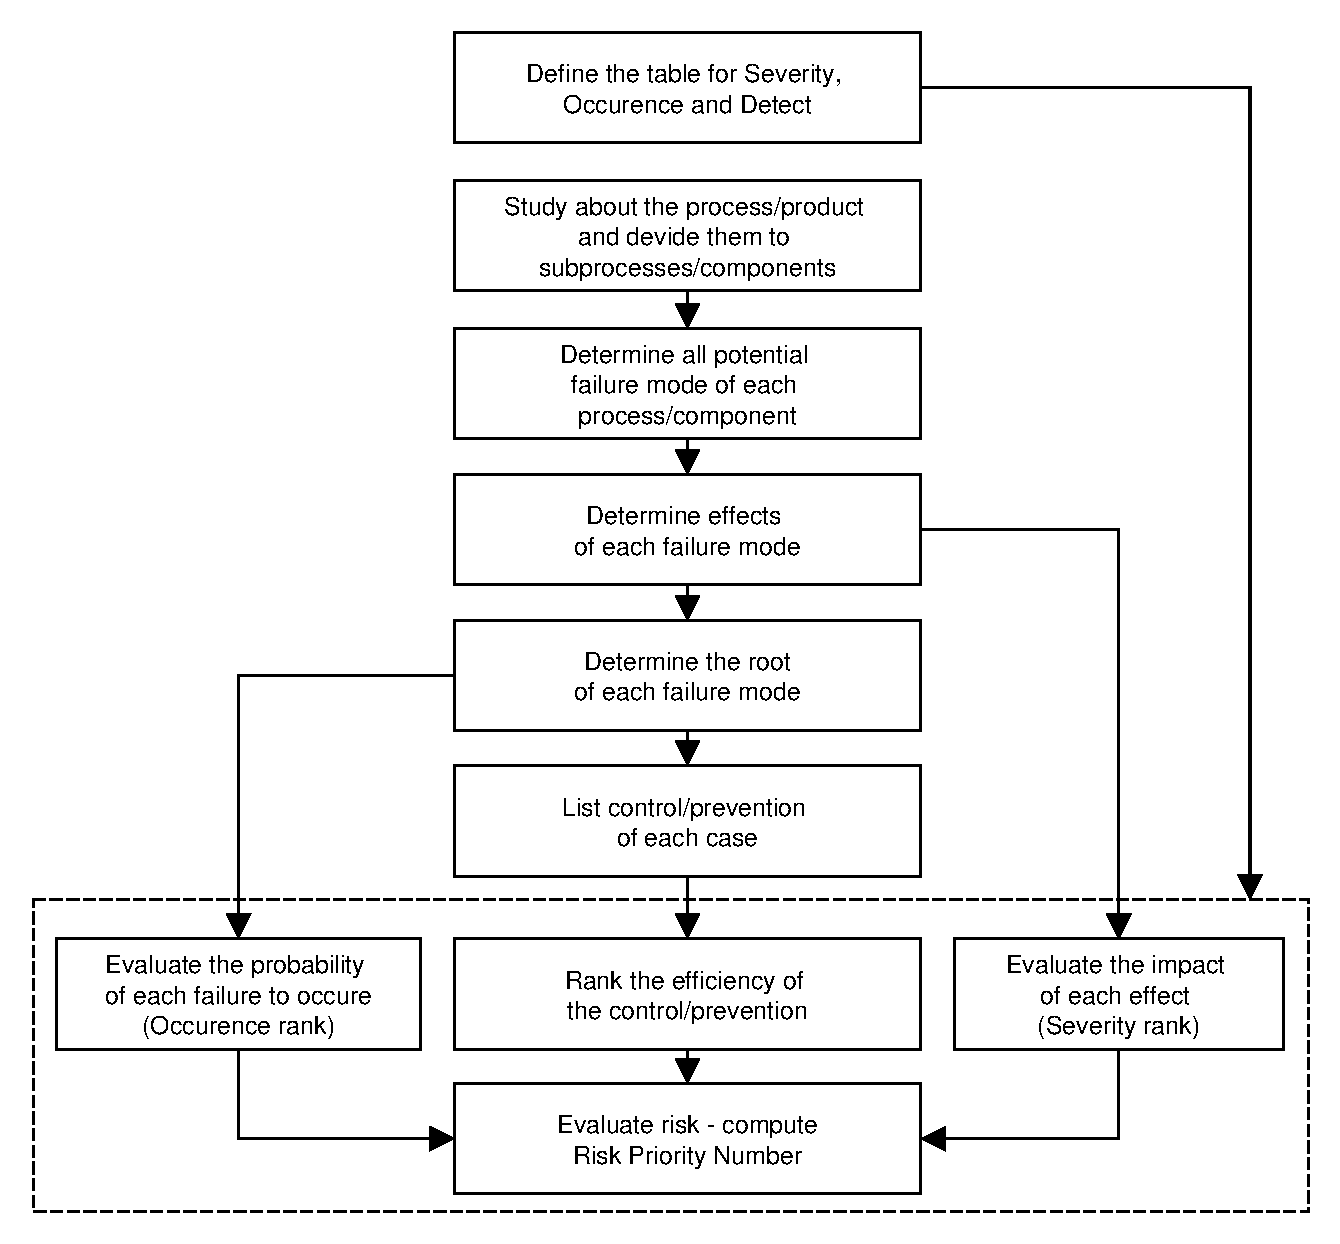
\includegraphics[width=\textwidth, keepaspectratio, angle=0]
  {fmea_chart.pdf}
  \caption{The necessary steps for FMEA methodology}
  \label{fig:fmea_chart}
\end{figure}

FEMA involves reviewing as many components, assemblies, and subsystems as
possible to identify failure modes, and their causes and effects. It also
involves a lot of human resources: experts and practitioners in particular
industrial fields \cite{tague_quality_2010}.
That is why this tool is considered as a relatively expensive approach, and is
adapted mostly for life-critical systems, related to military area, automotive,
gas and oil industry, health-care and life-support activity. There are other,
less costly but yet similar knowledge based analytical approaches, presented in
literature, for instance the adapted for industrial use Process Mapping
\cite{what_is_a_process_map}, and State analyses \cite{ruiz_state_2000}.


\subsection{Mean Time Between Failures} 

Mean time between failures (MTBF) is a statistical mean value for error-free
operation (between two failures) of an electronic device during the normal working life. The MTBF does not apply
to an individual component, it always refers to the phase with constant failure
rate (i.e. without early or wear failures). The higher the MTBF, the less often
the component fails and the more reliable it is. In addition to the MTBF value, the
environment and operating conditions should be taken into consideration. If a
device is operated under conditions beyond its specification (e.g. at extremely
high ambient temperatures or subject to a massive EMC load), then the MTBF
values are no longer valid and large numbers of failures might occur.

This term is based on the assumption that when a failure occurs, the system does
not generally remain in the down state, but is renewed or repaired. The time
required for renewal or repair (i.e. from the start of the down state to the
restoration of the up state) is known as  the Mean Time to Repair (MTTR), often
also called  Mean Down Time (MDT). These characteristics are the most common
parameters related to reliability which are provide by manufactures in the
documentation for their equipment.

As an instance, the Table \ref{tbl:siemens_mtbf} shows some values MTBF for the
equipment used in the previously described system. This data are provided by the
manufacture \cite{siemens_mtbf}.

\begin{table}[t]
\caption{MTBF values for some SIEMENS Simatic components}
\centering
	\begin{tabular}{l l r}
	\\	
	Part Number & Type Description & MTBF (years) \\
	\hline 
	6ES7321-1FF01-0AA0	& 8 Pt. AC Input	& 5,4 \\
	6ES7314-1AC00-0AB0	& CPU 314	& 22,2 \\
	6ES7321-1BH00-0AA0	& SM 321, DI 16 x DC24V	& 28,0 \\
	6ES7331-7NF00-0AB0	& AI 8 channels	& 76,0 \\
	6ES7951-0FD00-0AA0	& Memory Card	& 90,2 \\
	6ES7322-1BH01-0AA0	& DO 16 x DC 24V, 0,5 A	& 105,7 \\
	6ES7340-1AH01-0AE0	& CP 340	& 278,3 \\
	6ES7960-1AA04-5AA0	& Patch cable 1m	& 394,9 \\
	6ES7964-2AA04-0AB0	& DP-interface module	& 703,4 \\
	6ES7972-0BA12-0XA0	& profibus connector	& 19120,4 \\
	6ES7368-3BB00-0AA0	& Cable	& 317097,9 \\
	\hline
	\end{tabular}
	\label{tbl:siemens_mtbf}
\end{table}


\subsection{Knowledge-based Databases}

It is common that hardware vendors provide some parameters as MTBF for their
equipment, but there is no information about complex types of failures. Since
each relatively big manufacture usually has it is own history records for the
equipment, an idea to unite such historical data seems to be a relevant
responses to the problem. There exists international initiatives which gather
the data collected by users of equipment in a centralized database, in order to provide realistic data about
different types of technological devices. For example, plant and equipment
taxonomies developed by the Process Reliability Database Project (PERD)
\cite{reliabililty_database}.


\subsection{Safety standards {IEC 61508/IEC 61511}}

These standards is the quantitative approach for the failures analysis.  
They define a concept of functional safety as a safety instrumented
function calculated for electrical, electronic and programmable electronic systems.
The standards require a quantitative proof for the risk, based on calculating
the probabilities of dangerous failures. This calculation is carried out for the
complete safety loop, consisting of sensor, PLC and actuator. The standards
define the following steps for evaluation of safety:
\begin{itemize}
  \item Risk definition and assessment according to detailed probabilities of
  failure from sensor over controller to actuator for the overall component life
  time 
  \item Specification and implementation of measures for risk reduction
  \item Use of suitable instrumentation (evaluated or certified) 
  \item Periodic test for correct operation of the safety functions
\end{itemize}
Some of the calculated parameters are following:
\begin{itemize}
  \item Percentage of failures without the potential to put the safety-related system into a dangerous 
or fail-to-function state
  \item Average probability of failure on demand
  \item Failure rate for all safe detected failures
  \item Failure rate for all safe undetected failures
  \item Failure rate for all dangerous detected failures
  \item Failure rate for all dangerous undetected failures
\end{itemize}
The calculations are made for every single component of a system. 
Clearly, a complete quantitative evaluation can be determined only for
relatively simple and small devices, such as film resistors, transistors, relays
and etc. Characteristics of complex components such as processors and memory for
PLC are determined partially.

The complexity of the underlining approach for these standards and a
corresponding high cost restricts its application only for so-called Safety
Instrumented Systems (SIS) that are designed and used to prevent or mitigate
hazardous events, to protect people or the environment or prevent damage to
process equipment.
% For additional infor read this: 
% http://www.samson.de/pdf_en/w02360en.pdf

\subsection{Simulation}

Simulation is the imitation of the operation of a real-world process or system
over time\cite{banks_introduction_1999}. In industrial practice it is used as
the imitation of the real-life technological processes and equipment. It usually
includes generation of a software model which reflects the supposed system's
behaviour. It is also a common case when simulations involve hardware devices
and entire subsystems, such as networks, sensors and actuators, and even real
physical objects and media. Either existing and conceptual systems can be
modeled with simulation. The main goal of simulations is validation of system's
behaviour while a real system is not accessible, it is being designed, or it may
be dangerous to use its processes and machines. Examples of simulation approach 
can be found in performance optimisation \cite{tamimi_simulation_2012},
scientific modeling \cite{sharda_best_2011}, analysis of possible failures
\cite{weatherford_simulation_2003} and of failure avoidance
\cite{warrington_modelling_2002}.

The main issue of this approach is how an imitated system is close to the
corresponding model, i.e. how the quality and quantity of information provided
for the simulation reflects the processes and machines' behaviour in the real
life.

\subsection{Formal methods}

The Failure Mode and Effect Analysis is the first step of a system reliability
study. The Simulation can augment this analysis with a reality-like experience
of failures and of how the automated system would behave. However, only formal
methods can ensure reliability of a manufacturing system design
\cite{holloway_why_1997}. Formal methods apply logic and mathematics to
development process of systems and their analysis during operations. The are
used for specification, development and verification of software and hardware.

The formal methods have been used in industrial automaton for a half of century,
providing distinct field of research, development and application, mainly
for control engineering due to its importance. Nowadays, formal methods have
their own design programming languages as  \cite{spivey_z_1992} for instance,
and tools as \cite{event_b_web}, \cite{atelier_b_web} and \cite{nusmv} for
example.

\begin{figure}[th]
  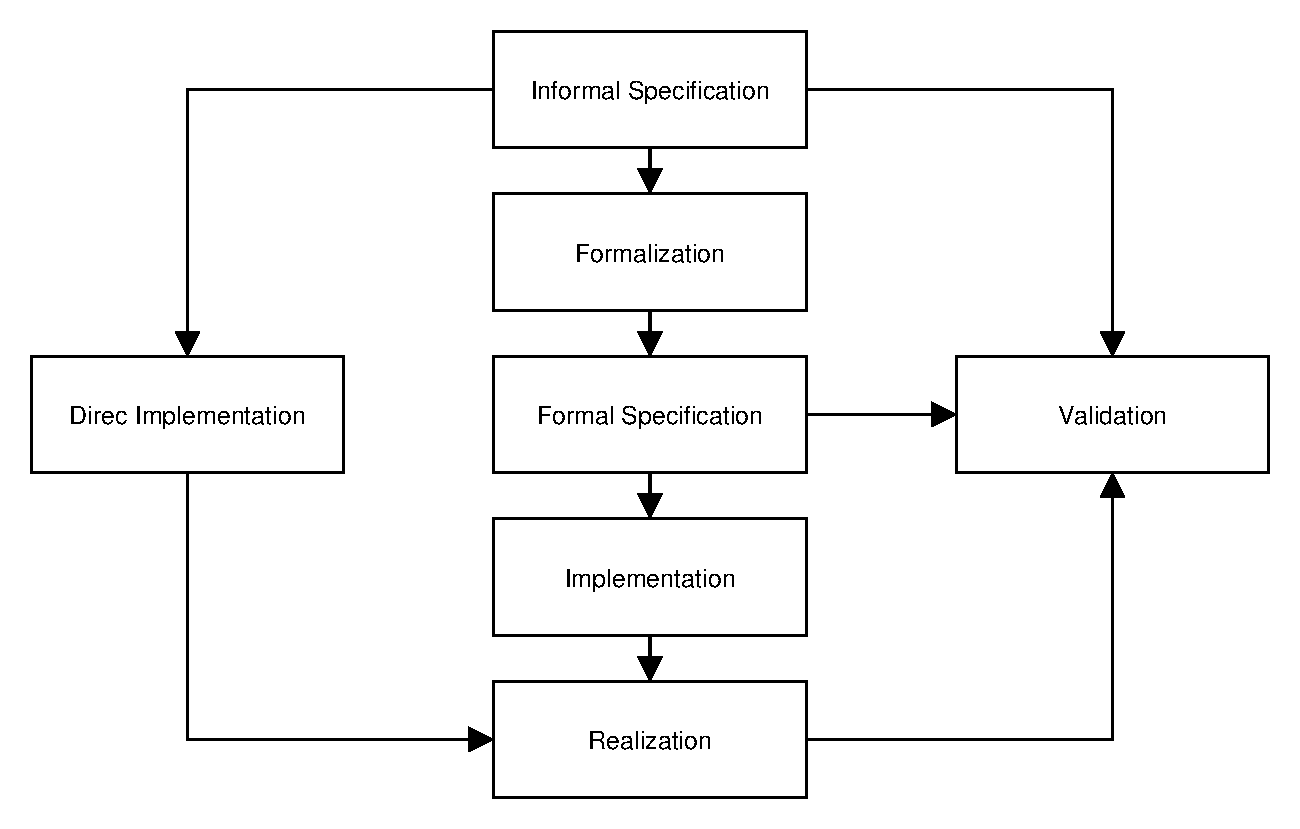
\includegraphics[width=\textwidth, keepaspectratio, angle=0]
  {forma_methods_in_design.pdf}
  \caption{Design process of automated systems}
  \label{fig:forma_methods_in_design}
\end{figure}

The Figure \ref{fig:forma_methods_in_design} depicts a generic model of a
manufacturing system design process. The design process of a particular system
starts, in most of the cases, with informal description of technological
processes. It specifies the system's behaviour in not a strictly semantically
and syntactically defined form. Additionally to the verbal form, the description
includes P\&I diagrams, equations and algorithms expressed in block diagrams.
The main problem with informal specifications is that they do not facilitate
tests for completeness, unambiguity and consistency of the system.

Until nowadays, the common approach is when after the stage of informal
specification immediately begins its direct implementation into a
code for {PLC} with a programming language. Instead, when applying formal
methods, the implementation stage follows after formalization of informal
descriptions into formal specification. Formalisation is performed by
humans, and involves conversion of textual and graphical information into the
form of a formal language or another representation (for instance, automata).

Formal specifications can be translated directly into programming languages
\cite{maclay_click_2000} by a design tool. This step eliminates the error prone
interpretation by humans ensuring that the system will behave exactly as it
was specified.

Formal specification of the system brings opportunity to apply 
\emph{verification} techniques to the design process. Verification is used
to prove some properties of the system's specification. These properties are
independent from the modeled system, such as, for example, existence of
deadlocks in the discrete-event systems approach.
Verification is closely related to \emph{Model checking} ``technique for
verifying finite state concurrent systems such as sequential circuit designs and
communication protocols. It has a number of advantages over traditional
approaches that are based on simulation, testing, and deductive
reasoning''\cite{clarke_model_1999}. Model checking verification considers a
system as state-based model specified using, for instance, automata framework,
and specifications of properties written in temporal logic.

A formal verification approach can be a model based or non model based. In 
model based approaches a model of the studied object is included into analysis.
This can be a model of technological process or of manufacturing equipment. In
non model based approaches the formal representation of specifications does not
include a model of the object. These approaches assume that, literally,
everything can happen. An example of this approach is development of a system
with a few formally described controllers, where the whole system, i.e. the
composition of the concurrent acting controllers needs to be verified for
deadlocks absence.

Due to importance of the problem of failures analysis for modern complex
automated systems, formal method tools are widely used to support it.
Whenever the specification of a system is accessible in a formal form, many
formal approaches can be applied for offline failure analyses of the system's
design and its online failures monitoring during its operation. 

The next Chapter \ref{chap:framework} describes an UML model based 
modeling approach for manufacturing systems design, and how this approach is
used to reflect failures, such that it is suitable for formal analysis due to
exploiting the automata framework at the internal layer. Then the
mathematical notation for discrete event systems is briefly presented,
different definitions of diagnosability are given, as well as an idea
underlining a new notion of diagnosability which is described in details in the
following Chapter \ref{chap:theory}.



\ifx \definition \undefined
	\newtheorem{definition}{Definition}
\fi
\ifx \conjecture \undefined
	\newtheorem{conjecture}{Conjecture}
\fi

\chapter{Diagnosis-oriented Modeling and Verification Framework}
\label{chap:framework}

This first part of the chapter presents a modeling approach for design of
manufacturing systems which exploits idea of decomposition of a system into modules, and presents them
in a form of UML blocks. It is shown then, how the modules are
represented internally by automata, and how the failures can be modeled. The
second part of this chapter gives a necessary introduction into a formal
notation for discrete event systems in terms of languages and automata,
and describes different types of diagnosability.

\section{Modeling Framework}

\subsection{Introduction}

The fundamental principle ``divide and concur'' underlies many techniques and
approaches either used solely at the level of individual engineers and
programmers or developed at the level of international standard committees and
organisations. For instances, one can recall object-oriented concepts in
traditional programming principles \cite{farrell_object-oriented_2013}, and
standards of International Electrotechnical Commission (IEC), particularly the
legacy IEC 61131-3 \cite{otto_iec_2009} which defines programming languages for
programmable logic controllers (PLC), and the modern IEC 61499
\cite{vyatkin_iec_2009} which represents a component solution for distributed
industrial automation systems aiming at portability, reusability,
interoperability and reconfiguration of distributed applications.

Many Integrated Development Environments (IDE) used in industrial world satisfy
all the requirements and standards in order to facilitate the process of
development, enrollment and maintenance of a complex system. They exploit
object-oriented concepts as classes with their instances, inheritance and
encapsulation (for instance, as in  \cite{serna_design_2010},
\cite{steinegger_design_2013} and \cite{zoitl_guidelines_2013}). However, these
concepts were not initially created bearing in mind the purpose of formal
verification. As a consequence, the tools widely used in industry nowadays do
not generally support approaches for DES raising in the scientific world. As a
response for the growing demand for intersection of classical development
process with formal techniques many researches attempt to create instrumental
and theoretical bridges. The most promising results seem to be reached in
formalizing Unified Modeling Language (UML), Statecharts, and general purpose
programming languages as C.

\begin{figure}[t]
	\centering
	\includegraphics{uml_state_machine.png}
	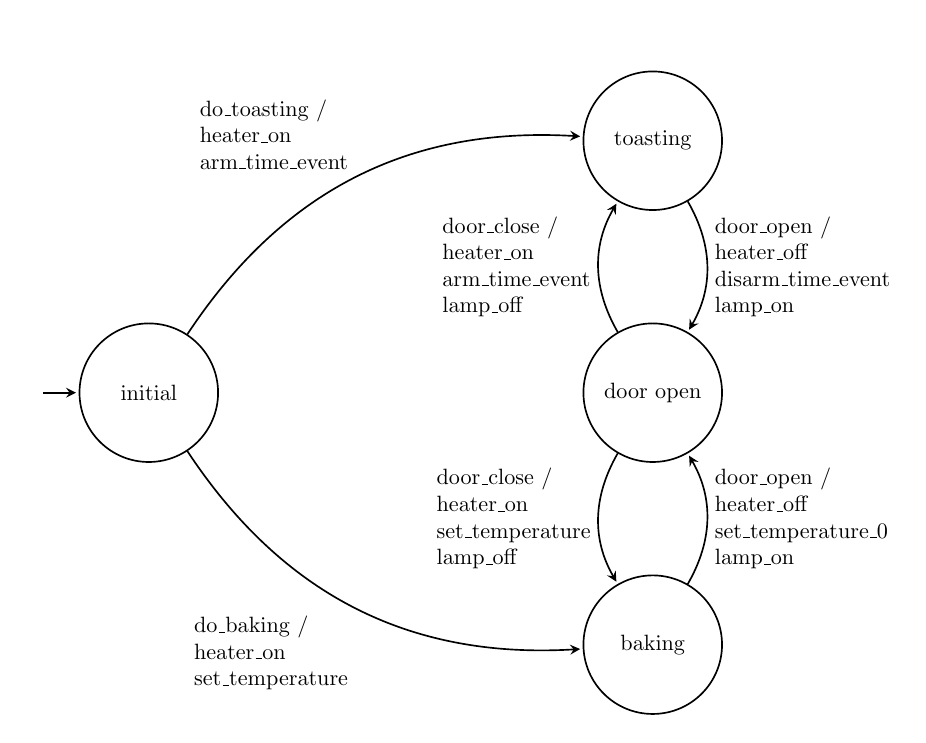
\begin{tikzpicture}[->,>=stealth, node distance=4cm, auto, shorten >=1pt,
	semithick, initial text=,	
		every node/.style={scale=0.8},
		every state/.style={minimum size=2.2cm},
	    accepting/.style={double distance=1.5pt, outer sep=0.75pt+\pgflinewidth}
	    ]
% \draw[help lines] (0,0) grid (6,2);
	\node[state]         (1) [] 	  {toasting};
	\node[state]         (3) [below of=1]       {door~open};
	\node[state]         (2) [below of=3]       {baking};
	\node[] (0') [left of=3] {}; %dummy
	\node[initial,state] (0) [left of=0']{initial};
	\node[above = 1em of 1] {}; %adds some space above
	\path
	(0)	edge [bend left, align=left]  node [above left]
		{ do\_toasting / \\ heater\_on \\  arm\_time\_event	}
	(1) 
	(0)	edge [bend right, align=left]  node [below left] 
		{ do\_baking / \\ heater\_on \\ set\_temperature }
	(2)
	(1)	edge [bend left, align=left]  node [right]
		{ door\_open / \\ heater\_off \\ disarm\_time\_event \\ lamp\_on }
	(3) 
	(3)	edge [bend left, align=left]  node [left]
		{ door\_close / \\ heater\_on \\ arm\_time\_event \\ lamp\_off }
	(1) 
	(2)	edge [bend right, align=left]  node [right]
		{ door\_open / \\ heater\_off \\ set\_temperature\_0 \\ lamp\_on }
	(3) 
	(3)	edge [bend right, align=left]  node [left]
		{ door\_close / \\ heater\_on \\ set\_temperature \\ lamp\_off }
	(2) 
	;
	\end{tikzpicture}

	\caption{Example of an UML Statechart diagram (at top) and its representation
	by the Mealy automaton}
	\label{fig:example_of_UML_with_Mealy}
\end{figure}

In \cite{mcumber_general_2001} the authors introduce a framework which allows to
convert an UML model into the formal languages described in the form of
specification. The framework can be applied only for a subset of UML diagrams.
The resulting formal specification can be used for model checking and
simulation, using existing tools aimed for this purpose. Figure
\ref{fig:example_of_UML_with_Mealy} depicts the instance of an UML diagram and
its representation by a Mealy automaton which, in its turn, can be transformed
into a classical automaton. In \cite{bonfe_design_2003} the authors develop a
framework to transform UML diagrams and Statecharts into Computation Tree Logic
(CTL) which is the used in a model checking tool.
Other works to mention are \cite{dong_model_2001}, where UML diagrams are mapped
to automata, \cite{frey_re-engineering_2004} where the authors concentrate on
converting PLC languages to UML and then to automata. Even a such known widely
spread tool as Matlab \cite{matlab}, used by both practitioners and
theoreticians, also has to be tweaked in order to get its modeling ability
closer to a formal representation. Examples of such attempts are
\cite{ray_automated_2007} and \cite{li_stateflow_2011}. An instance of model
checking tool, which is exploited by many of the approaches mentioned above, the
most notable one is NuSMV \cite{nusmv} which automatically verifies properties
of finite-state systems, expressed in CTL, Linear Temporal Logic (LTL) or
Property Specification Language (PSL).

Quick analysis of the aforementioned attempts to bridge the most widely
used object-oriented IDEs and their underlining modeling technologies shows that
they solve the problem of using formal methods by system's developers
only partially. The reason is, as it was said before, that those concepts
and tools had been developed before formal methods became useful in practice,
and they simply can not be merged with modern formal approaches. The problem
lays, firstly, in the ambiguity of legacy methods, their freedom of
interpretation. It appears when, for instance, one tries to convert an UML
diagram to automata. Second, the problem comes from the fact, that producers of
development tools have created a wide range of derivatives of one standard,
which, at one hand, satisfied requirements of the market and, on the other hand,
made these implementations incompatible to each other. Now, when formal
approaches both, have reached enough theoretical level, and have growing demand
due to the high complexity of currently appearing systems, there is a need for
new approaches and tools that exploit formal methods as an underlying concept.

One of the approaches which uses the object-oriented principles, and focuses on
formal verification is presented in \cite{sartini_architectures_2010}. The
approach introduces a modeling entity called \emph{Generalized Device} and shows
how it can be used for formal verification in the DES framework. The approach is a
refined architecture of a concept of \emph{Generalized Actuator} for industrial
automated systems \cite{faldella_hierarchical_2008}. The next section gives a
brief introduction into both the concept and the refined approach.


\subsection{Generalized Actuator and Generalized Device}

\subsubsection{Generalized Actuator}

The GA approach aims to reduce complexity of the modeling process using
standardized object-oriented concepts of engineering.
An idea of GA is to identificate essential patterns in automated manufacturing
systems, and design control software entities suitable for formal methods of DES
theory. The GA approach gives a modeling framework and defines a design
procedure with following characteristics:
\begin{itemize}
  \item Encapsulation of ``actuation mechanism'';
  \item Hierarchical representation of a plant;
  \item Separation of control policies from actuation mechanisms in each GA;
  \item Support of visualization of plant's hardware;
  \item Interoperability and reusability of GAs.
\end{itemize}

\begin{figure}[!t]
	\centering
	\includegraphics[width=30em]{ga_blocks.png}
	\includegraphics[width=30em]{ga_automaton.png}
	\caption{GA with two types of interfaces (top) and its underlining
	formal representation by the automaton (bottom)}
	\label{fig:ga_blocks}
\end{figure}

The GA implements a concept of abstraction. It implies that all the actions of a
complex process, from the high-level point of view, can be decomposed into sets
of two kinds: \emph{Do-Done} actions and \emph{Start-Stop} actions.

The Do-Done GA reflects a process which starts by an external (with respect to
this process) ``Do'' command, and continues until an internal (with respect to
this process) decision to terminate is taken. The duration can be finite or
infinite. After its termination the process issues ``Done'' event. The 
instance of a process which can be abstracted by this type of GA is the opening
of a valve: the command ``Do'' is issued to open the valve; when it opens, the
event ``Done'' occurs.

The Start-Stop GA is an abstraction of a process which starts by an external
``Start'' event, and continues until an external ``Stop" event occurs .
Again, the duration can be finite or infinite. The instance of a such process is
a temperature regulation with a heater: the ``Start'' event switches on the
heater; when temperature reaches a required level the ``Stop'' event switches it off.

The above described two types of GA can be implemented as Functional Blocks
(FB) in terms of IEC 61131-3 standard, as depicted in Figure
\ref{fig:ga_blocks}
\footnote{The image is borrowed from \cite{faldella_hierarchical_2008}}. 
Besides the essential inputs and outputs necessary to perform the above described types of actions, the blocks have other inputs and
outputs related to the low level of processes, and to some additional
information related to the high level. 

Internally, each type of GA is represented by the automaton, as depicted on the
figure. Each state of the automaton can abstract a set of states of other
automata, i.e. GAs contain a hierarchical structure of automata.

A design procedure, according to the framework of GA can be described by the
following steps:
\begin{itemize}
  \item Identification of distinguished processes and their basic actions;
  \item Classification of actions into Do-Done and Start-Stop actions;
  \item Definition of GAs for two kinds of actions;
  \item Assigning low level information and additional information to each GA;
  \item Design of internal hierarchical structure and logic of automata for
  each GA.
\end{itemize}

The last two steps in the above described design procedure encapsulate a logic
specific for a given process. Potentially, the complexity of internal
implementations of GAs is not limited. Thus, the functional blocks
corresponding to the GAs can became very specific, such that it would be
possible to reuse them only at the same plant, or for a technologically similar
processes. A designer of a GA must be aware of this problem, and maintain
simplicity of the internal implementation. Instead of increasing the complexity
of internal structure of a GA, one can create other GAs. However, this
process relies solely on decision of a particular designer for a system.

The design problem, described above, can be reformulated as that a GA abstracts
a process at its high level, but does not abstract it at its low level. The
architectural approach of Generalized Device (GD) is aimed to solve this
problem.

\subsubsection{Generalized Device}

The idea of a Generalized Device is based of the observation that the most
of different low level field devices can be viewed as only two kind of abstract
devices: either single acting device or double acting device. Each kind
of devices has an actuator and also may have sensors.

A single acting device has only one command (input) to perform a ``forward'' or
``on'' action. The ``backward'' or ``off'' action is performed by the device
itself, implicitly ore explicitly. Examples of single acting devices are:
a cylinder with a return spring, a contactor itself or together with any
controlled equipment (electric motor, heater, lighting, etc).

A double action device has one command to activate the device and another
command to deactivate it. Simultaneous commands on inputs of the device are
usually prohibited or have now effect on a state of the device. The instances of
double action devices are: a double acting cylinder, an auxiliary relay or any
start-stop device which may itself be a composition of two single acting
devices.

The common feature of the both, single and double acting devices is that they
have two clearly distinguished states. In order to detect what the current state
of a device stays in, it is usually equipped with one or two sensors. In case of
two sensors each of them gives the feedback for the corresponding state. In case
of one sensor one level of its signal corresponds to the first state of the
device, another level - to the second one. A state of the device in the case
when it has no sensors is implied according to a previous command. Concluding,
a classification of the devices in this approach is the following:

\begin{itemize}
  \item Single acting device
	\begin{itemize}
	  \item with no feedback
	  \item with single feedback
	  \item with double feedback
	\end{itemize} 
  \item Double acting device
	\begin{itemize}
	  \item with no feedback
	  \item with single feedback
	  \item with double feedback
	\end{itemize} 
\end{itemize} 


\begin{figure}[t]
	\centering
% 	\includegraphics[width=30em]{dadf.png}
	\includegraphics[width=30em]{dadf.pdf}
	\caption{Device with Double Actuation and Double Feedback (DADF) and its
	connection to a physical device (valve)}
	\label{fig:dadf}
\end{figure}
 
As an instance, the Figure \ref{fig:dadf} depicts the device with double
activation and double feedback. It abstracts a physical device, the valve
in this example, for a higher level GA.

\begin{figure}[t]
	\centering
	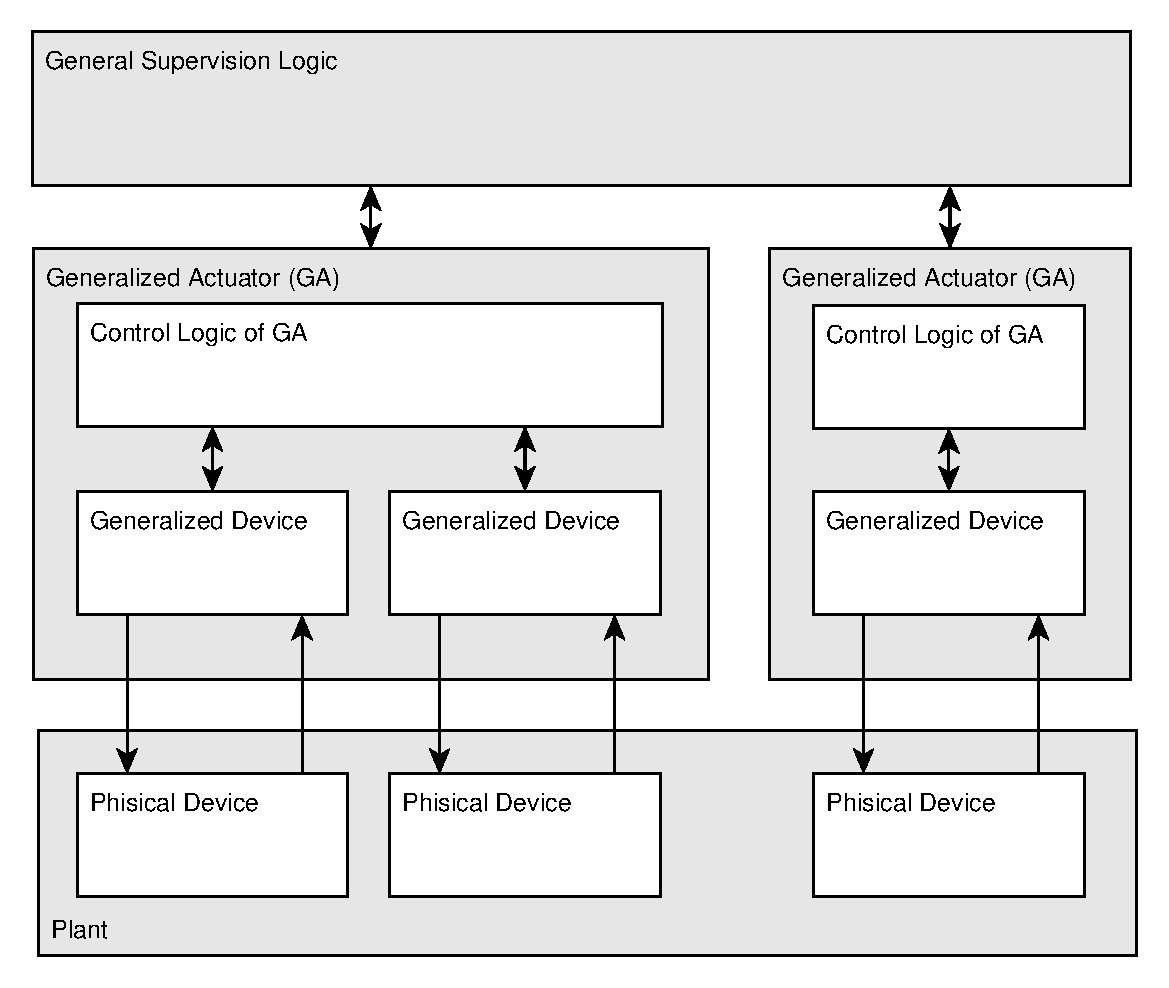
\includegraphics[width=30em]{levels_ga_gd.pdf}
	\caption{Hierarchical relation of system's components: high level logic of
	plant, GAs, GDs and physical devices}
	\label{fig:levels_ga_gd}
\end{figure}

The approach of generalized actuators and devices allows to construct complex
automated systems using simple predefined models, as it is shown at the Figure
\ref{fig:levels_ga_gd}.
  
Due to representation of the system's models by automata, various DES techniques
can be applied in order to define and solve control and diagnosis problems for
entire system. To preserve the level of abstraction, however,
additional information necessary for a required problem has to be encapsulated
into modules. Particularly, possible failure behaviour should be incorporated
into modules for the diagnosability problem.

The next section proceeds with a description of how the approach of generalized
device is used for modeling and analyses of faults.


\subsubsection{Generalized Device and Failures Diagnosis}

This section briefly describes an approach for building structured formal
models, presented in \cite{sartini_methodology_2010}. The methodology extends
the approach of generalized device to facilitate diagnosis verification
and monitoring problems. The authors present each GD as a composition of
automata, where automata reflect control logic and a model of physical device,
decomposed into sensors, actuators, components and their constrains. For the
sake of simplicity, the approach is presented further with a small illustrative
example. The example shows the idea of decomposition with two components of a
hypothetical device (think of a valve from the system given in Chapter
\ref{chap:problem_description}), their constrains and how failures are modeled.

\begin{figure}[t]
	\centering
	\includegraphics[scale=0.8]{do.pdf}
	\caption{Automaton representing digital output}
	\label{fig:do}
\end{figure}

The Figure \ref{fig:do} depicts a model of digital output (a
model of digital input would be equal). The automaton has two states,
reflecting the low and high levels of signal. The event labels of the automaton
are corresponding to digital signal states as shown in the table
\ref{tbl:do_events}. The states of a signal are treated as events because
they are seen as readings (two values) of a variable (either it is output or
input) in a program in PLC, while the cyclical program execution.

\begin{table}[t]
\caption{Correspondence of automata event labels to digital output signals}
\centering
	\begin{tabular}{l l}
	\\	
	Label & Digital output signal state\\
	\hline
	do\_lo & Digital output signal is low\\
	do\_hi & Digital output signal is high\\
	\end{tabular}
	\label{tbl:do_events}
\end{table}

\begin{figure}[t]
	\centering
	\includegraphics[scale=0.7]{./figures/relay.pdf}
	\includegraphics[scale=0.7]{do2relay.pdf} 
	\includegraphics[scale=0.7]{do+relay.pdf} 
	\caption{Automata models of Relay (top left, constrains (top right), and 
	result of composition (bottom)}
	\label{fig:do+relay}
\end{figure}

In major of cases, a digital output is linked to an actuator, there is an
intermediate signal amplifier, e.g. an electromagnetic relay. It acts also as an
galvanic isolation of the PLC and the field device. 

In this example, the behaviour of the relay is related to the behaviour of
digital output, i.e. it is constrained by the digital output. A model of the
relay, a model of constrain and the resulting composition of all the
aforementioned components is depicted in the Figure \ref{fig:do+relay}.

\begin{figure}[t]
	\centering
	\includegraphics[scale=0.7]{relay_f0.pdf}
	\caption{Failure model of the relay (example of the broken coil) }
	\label{fig:relay_f0}
\end{figure}s

For illustration of a failure lets pick one of the possible relays failures,
e.g. broken coil. The corresponding model of the relay with this failure is
depicted in the Figure \ref{fig:relay_f0} (event $f0$ states for the failure
event). Similar to the this failure, a ``stuck on'' relay's failure can be
modeled.

As the the approach of GD assumes, almost any field device can be decomposed
into simple components, as ones described in the above example. The failure
models for such components can be easily determined. More complex components can
be then composed by using the simple models and constrain automata. Thus, a
set of predefined models can be exploited for building a library of GD. Since
all the models include failure behaviour, formal diagnosability analysis
techniques can be applied.

In the Chapter \ref{chap:theory} a part of the work is devoted to an extension
of the above failure modeling approach such that a failure behaviour can be
modeled without failure events, by state marking. It will be shown how a failure
behaviour can be separated from a non-failure one automatically, for further
diagnosability analysis.
 

\section{Discrete Event Systems Framework for Diagnosability Verification}

\subsection{Introduction}

Discrete Event Systems (DES) are systems, the dynamic of which is characterized
by asynchronous occurrence of \emph{events}. An event is a fundamental concept
which can be viewed and described as ``something happened'', either in systems
designed by humans or in nature. Events have no property of continuation, they
are instant, and can be observed only at discrete points in time. The second
fundamental concept, characterizing a DES, is a state. A state is viewed as a
result of \emph{temporally ordered} discrete events, occurred starting from a
moment when the system was at its \emph{initial state}. The initial state of a
DES characterizes the system before occurrence of any event. In reality, this
characteristic may be seen as an assumption or ``agreement'' for the given
system. Being at a certain state, when an event occurs, the system makes a
\emph{transition} to another state.

The examples of events are: switching a light on, pressing a button, a 
moment of rising a temperature above a certain level. The corresponding states
are: the light is on, the button is down, the temperature is high.

Historically, all the system's events are thought as of an \emph{alphabet}.
Temporally ordered, they form \emph{words} which, consequently, form a
\emph{language}. At this level of abstraction DES are studied by the
\emph{language theory} \cite{aho_theory_1968}.

Formal language theory is closely related to \emph{Automata theory}
\cite{hopcroft_introduction_2007}. Automata are used as one of the modeling
formalisms for DES. A single automaton can be represented as a directed graph,
and it is, probably, the simplest way a complex system's behaviour can be graphically
and formally described and conceived by humans.

The next section gives the preliminaries from theories of languages and
automata, used in this document.


\subsection{Notation}

The notation used in this document is the one in
\cite{cassandras_introduction_2010}. For the benefit of the reader we place here
the most essential notation necessary for understanding of the further material.

Let $\Sigma$ be a finite set of events. A sequence of events is a string.
$\Sigma^*$ denotes a set of all finite strings over $\Sigma$.
$L\subseteq\Sigma^*$ is a language over $\Sigma$. Given strings $s$ and $t$,
$st$ is their concatenation. Given strings $s$ and $w$, $w$ is a prefix of $s$
if it exists $t$ such that $wt = s$. Prefix closure of $L$, denoted by
$\overline{L}$ is a set of all prefixes of all the strings in $L$.
If $\overline{L} = L$ then $L$ is prefix-closed. The post language of $L$ after
a string $s$ is denoted as $L/s$, i.e. $L/s := \{t\mid st \in L\}$. We
write $\sigma \in s$ if the event $\sigma \in \Sigma$ appears in the string $s
\in \Sigma^*$. If $\{s\}$ is a singleton, we write $s$ for operations on
languages.

An automaton $G$ is a tuple $$G := \left< X,\Sigma,\delta,x_0, X_m \right>,$$
where $X$ is a set of states, $x_0 \in X$ is an initial state, $X_m \subseteq X$
is the set of marked states, and $\delta: X \times \Sigma \rightarrow X$ is the
transition function.
We say a language $L := \mathcal{L}(G)$ is generated or recognized by the
automaton $G$. In this paper we assume that for each language there is always a
corresponding automaton, and vice versa. The marked language $L_m \subseteq L$
is intended to make a part of the automaton's behaviour distinguishable in a
certain context.

Some events of DES can not be observed. To reflect that the set of events
$\Sigma$ is partitioned into disjointed sets of observable events $\Sigma_o$ and
not observable events $\Sigma_{ou}$, i.e. $\Sigma = \Sigma_o~\dot{\cup}~
\Sigma_{ou}$.
$M: \Sigma^* \rightarrow \Sigma_o^*$ denotes natural projection that
erases unobservable events.
% ; $\epsilon$ means the empty string. 
The corresponding inverse projection is $M^{-1}: \Sigma_o^* \rightarrow
2^{\Sigma^*}$.

Let $I := \{1,2,\ldots,n\} \subset  \mathbb{N}$ be an index set. A system is
defined by a set of automata $\{G_{i \in I}\}$ and a corresponding set of
languages $\{L_{i \in I}\}$. We use the term \emph{local} in context of the
automata and languages from these sets. The \emph{global} language of the system
is defined by the parallel composition \cite{cassandras_introduction_2010} of
its local languages:
$L := \parallel_{i \in I} L_i$.
The natural projection for the local languages is defined as 
$P_i := \Sigma^* \rightarrow \Sigma_i^*$. We extend it to the system's languages
as follows: $P_i(L) := \{s\mid s\in L_{i}\}$, and 
$P_i^{-1}(L_{i}) := \{s \mid s \in L, P_i(s) \in L_i\}, ~i \in I$.
We also define natural projection over observable events for the index set: 
$M_i :\Sigma_i^* \rightarrow \Sigma_{i,o}^*$, natural projection over common
events:
$P_{i,c} : \Sigma_i^* \rightarrow (\Sigma_i \cap \bigcup_{j\neq
i}^I\Sigma_j)^*$, and natural projection over observable and common events:
$P_{i,co} : (\Sigma_i \cup \Sigma_o)^* \rightarrow (\Sigma_{o} \cup (\Sigma_i
\cap \bigcup_{j\neq i}^I\Sigma_j))^*$. All the above projections, as well as
the corresponding inverse projections, are defined also for languages in the
usual manner.


\subsection{Abstraction by decomposition}

For model checking and verification of DES the state explosion problem is one of
the main limitations for their application in industry. The most important
technique to deal with the state explosion problem is abstraction. The basic
idea of abstraction is that some parts of a given system \emph{do not have
effect} on particular properties, and hence, these parts can be
\emph{eliminated} from the system's design.

One of the most effective abstraction techniques, compositional reasoning
\cite{berezin_compositional_1998}, deals with complex systems in order to reduce
its complexity by breaking into smaller parts, checking its properties and then
deducing the system correctness. These parts do not necessary reflect the real
structure of a system if any. On the other hand, the most of systems are
already structured in reality. Their structure is understood by humans, the
properties of their parts can be described and checked easier relatively to the
complex system. Then the models of the system's parts along with their
properties can be reused.

The modeling approach, described in this chapter, exploits automata framework
and, which makes the idea of abstraction applicable for it.

% theories, and is mainly oriented for industrial use .by applying the design patterns for and verification of system's properties. The approach
% exploits automata and language theories, and is mainly oriented for industrial
% use.

% When a system is built from its components, the state explosion problem rises on
% the parallel (synchronous) composition of component's models. Then it seems
% rational to modify the description of a complex system such that a parallel
% composition of component's models can be avoided, and tune the analysis
% techniques to suit the new description.


\section{Diagnosability of DES}

In Discrete-Event Systems, diagnosis of a fault is a problem of deciding whether
or not the fault occurred, under partial observation of the system's events.
The problem was defined in \cite{sampath_diagnosability_1995} where the authors
consider a monolithic model of a system. This definition and new definitions
of diagnosability problem, emerged later, may be grouped as it is make, for
example, in \cite{su_global_2005}, where an approach can be centralized as in
\cite{sampath_diagnosability_1995}, \cite{jiang_polynomial_2001} and
\cite{yoo_polynomial-time_2002}, 
decentralized as in \cite{debouk_coordinated_1998},
\cite{pencole_formal_2005} and \cite{qiu_decentralized_2006}, 
or distributed as in \cite{su_distributed_2002}.
The centralized and decentralized approaches require building of a monolithic
model. This process corresponds with exponential growth of the model's state
space, which makes the diagnosability problem intractable for complex large
systems with high modularity.

Architectures for on-line diagnosis can be categorized as follows:
centralized, decentralized and distributed.


\begin{figure}[th]
\centering
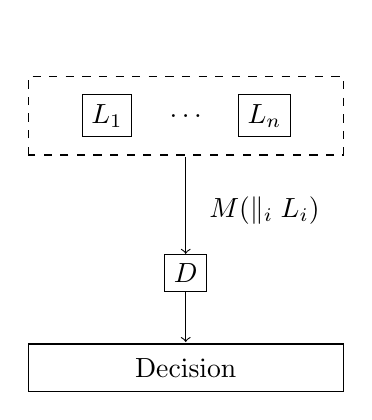
\begin{tikzpicture}
	\node[draw]		(0)	at (1, 3) 		{$L_1$};
  \node[] (fake) [above of=0]              {}; %for space above the picture
	\node[]			(1)	[right of = 0]	{$\ldots$};
	\node[draw]		(2)	[right of = 1]	{$L_n$};
	\draw[dashed] (0, 2.5) rectangle (4, 3.5);
	\node[]			(3) at (2, 2.6) {};
	\node[draw]		(4) at (2, 1) {$D$};
	\draw[->] (3) -- (4);
	\node[]	at (3, 1.8) {$M(\parallel_{i} L_i)$};
	\node[]		(5) [below of = 4] {};
	\draw[->] (4) -- (5);
	\draw[] (0, -.5) rectangle (4, 0.1);
	\node[]			(3) at (2, -.2) {Decision};
\end{tikzpicture}
\caption{Architecture of a system with centralized diagnosis}
\label{fig_centralized}
% \end{figure}
% 
% \begin{figure}[t]
% \centering
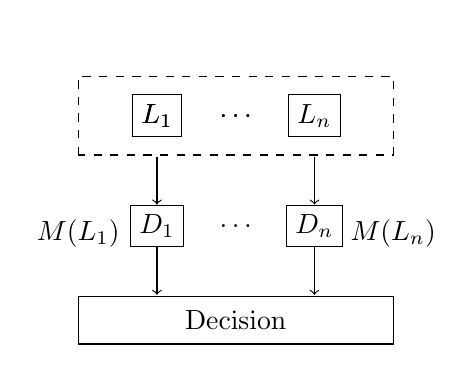
\begin{tikzpicture}
	\node[draw]		(0)	at (1, 3) 		{$L_1$};
   \node[] (fake) [above of=0]              {}; %for space above the picture
	\node[]		(0)	at (1, 3) 		{$L_1$};
	\node[]			(1)	[right of = 0]	{$\ldots$};
	\node[draw]		(2)	[right of = 1]	{$L_n$};
	\draw[dashed] (0, 2.5) rectangle (4, 3.5);

	\node[]			(000)	at (1, 2.6) {};
	\node[draw]		(00) [below of = 000] {$D_1$};
	\node[]			(10) [below of = 00] {$$};
	\draw[->] (000) -- (00);
	\draw[->] (00) -- (10);

	\node[]			(1)	[right of = 0]	{$\ldots$};
	\node[]			(11)[right of = 00]	{$\ldots$};

	\node[]			(222)	at (3, 2.6) {};
	\node[draw]		(22) [below of = 222] {$D_n$};
	\node[]			(20) [below of = 22] {$$};
	\draw[->] (222) -- (22);
	\draw[->] (22) -- (20);

	\node[]	at (0, 1.5) {$M(L_1)$};
	\node[]	at (4, 1.5) {$M(L_n)$};

	\draw[] (0, 0.7) rectangle (4, 0.1);
	\node[]			(3) at (2, .4) {Decision};
\end{tikzpicture}
\caption{Architecture of a system with decentralized diagnosis}
\label{fig_decentralized}
\end{figure}

\begin{figure}[t]
\centering
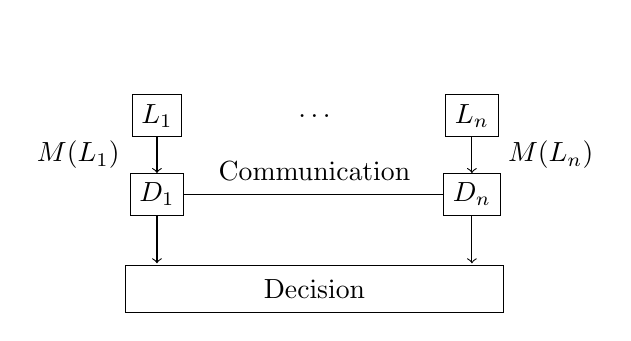
\begin{tikzpicture}
	\node[draw]		(0)	at (1, 2) 		{$L_1$};
  \node[] (fake) [above of=0]              {}; %for space above the picture
	\node[draw]		(00) [below of = 0] {$D_1$};
% 	\node[draw]		(p0) [below of = 00] {Decision$_1$};
	\node[]			(10) [below of = 00] {};
	\draw[->] (0) -- (00);
	\draw[->] (00) -- (10);

	\node[]			(1)	at (3, 2)	{$\ldots$};
	\node[] at (3, 1.3) {Communication};

	\node[draw]		(2)	at (5, 2) 		{$L_n$};
	\node[draw]		(22) [below of = 2] {$D_n$};

	\draw[] (.6, 0.1) rectangle (5.4, -0.5);
	\node[]			(3) at (3, -0.2) {Decision};

% 	\node[draw]		(p2) [below of = 22] {Decision$_n$};
	\node[]			(20) [below of = 22] {};
	\draw[->] (2) -- (22);
	\draw[->] (22) -- (20);
	\draw[] (00) -- (22);

	\node[]	at (0, 1.5) {$M(L_1)$};
	\node[]	at (6, 1.5) {$M(L_n)$};
\end{tikzpicture}
\caption{Architecture of a system with distributed diagnosis}
\label{fig_distributed}
\end{figure}

\subsection{Centralized diagnosability}
This architecture refers to a global model (language).If the system is modular,
then the global language is built by the parallel composition of the local
languages. All the observations are performed at one site. In this architecture
only one diagnoser $D$ \cite{sampath_diagnosability_1995} is constructed. Upon
the current state of the diagnoser a decision on the fault occurrence is made.
The structure is depicted in Figure \ref{fig_centralized}.

\subsection{Decentralized diagnosability}
This approach also exploits the entire model of a system built from its modules,
but several local sites perform observations using only local diagnosers.
The diagnosers do not communicate to each other, but they provide necessary
information (via a protocol) to a central decision node. This architecture is
depicted in Figure \ref{fig_decentralized}.

\subsection{Distributed diagnosability}
The architecture is depicted in Figure \ref{fig_distributed}.
The distributed approach does not require to built the entire model of the
system. The architecture implies that the system has a set of observation spots,
and each spot observes only one module of the system. A communication among
observation spots is possible in order to make a decision about a fault
occurrence.

% In \cite{basilio_computation_2012} the authors search for a
% minimal even-base, e.g. a minimal set of observable events, that ensures
% diagnosability for a given language (module).

The notion of modular diagnosability meets the same architectural implications,
and we refer to it as to the distributed approach when the amount of information
the observation spots communicate to each other is equal to zero. 

For the distributed approach, in general, the bigger the observation spots for
the same system, the less communications among the spots is required.
Figure \ref{fig:curves} shows that the average size of a composed module grows
while the system's modules are composed together (we imply that each module is
represented by automata, and the size of a module is reflected by the number of
states of a corresponding automaton).
The shape of this curve depends mostly on the order the modules are taken for
the composition, but the initial point, when the system has maximal modularity,
and the final point, when all the modules are composed into one monolithic
model, remain the same. Assuming that the system is diagnosable, the average
size of a diagnoser grows much faster, since it is exponential with respect to
the average size of a module, in the worst case.
The amount of events the diagnosers have to exchange among each other, in order
to decide if a fault occurred, is decreasing. The reason the diagnosers require
less event for decision making is due to the fact that they become more
self-sufficient, since amount of observable events available for each
diagnoser without communications is growing. Thus, the events exchange rate
decreases down to the point where no communications is required to make a
decision about the faults occurrence. That is the point when the system becomes
modular diagnosable (the notion of modular diagnosability was introduced in
\cite{contant_diagnosability_2006}). The following composition of the modules
does not affect diagnosability, and leads only to the growth of the modules' and
diagnosers' sizes.

In our approach, given a system with an initial natural modularity, we search
for a point, when the system is modular diagnosable. If the system is diagnosable,
then this point can always be found. The modules corresponding to that
modularity we call \emph{virtual}, since they differ from natural modules and
used only to build diagnosers.

\begin{figure}[t]
\centering
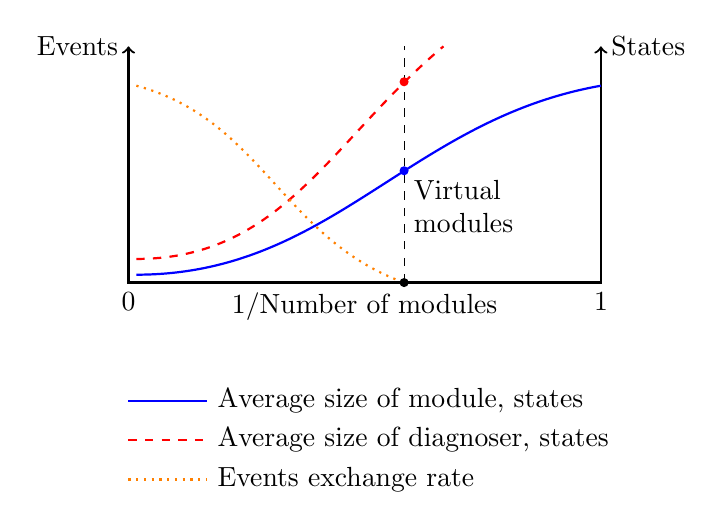
\begin{tikzpicture}
% \draw[help lines] (0,0) grid (5,3);
% Axis 
\draw [thick, <->] 
	(0,3) node[left]{Events} -- 
	(0,0) node[below]{0} -- 
	(6,0) node[below]{1} -- 
	(6,3) node[right]{States};
\node [below] at (3,0) {1/Number of modules};
% Curve of the average size of modules
\draw[blue, thick] (0.1,.1) to [out=0,in=-170] (6,2.5); 
% Curve of the average size of diagnosers
\draw[red, thick, dashed] (0.1,.3) to [out=0,in=-140] (4,3); 
% Curve of the amount of communication
\draw[orange, thick, dotted] (0.1,2.5) to [out=-15,in=160] (3.5,0); 
% Line of the point with virtual modularity
\draw[dashed] (3.5,0) -- (3.5,3);
% Point of virtual modularity  
\draw [fill] (3.5,0) circle [radius=0.05];
\draw [fill, blue] (3.5,1.42) circle[radius=0.05] 
	node[align=left, black, below right] {Virtual\\ modules}; 
\draw [fill, red] (3.5,2.55) circle [radius=0.05];
% Legend
\draw[blue, thick] (0,-1.5) -- (1,-1.5)
	node[black, right] {Average size of module, states};
\draw[red, thick, dashed] (0,-2) -- (1,-2)
	node[black, right] {Average size of diagnoser, states};
\draw[orange, thick, dotted] (0,-2.5) -- (1,-2.5) 
	node[black, right] {Events exchange rate};

\end{tikzpicture}
\caption{Size of modules, diagnosers, and events exchange rate, changing 
with respect to the degree of modularity of the system}
\label{fig:curves}
\end{figure}



\subsection{Diagnosability of a Modular System}

Diagnosability analysis uses a notion of a faulty language to describe the
faulty behaviour of a discrete-event system. This section discuses design issues
related to representations of the faulty language and focuses on a definition
of modular diagnosability.

The faulty behavior is usually modeled by introducing fault events or by faulty
specifications. We refer to this approaches as to \emph{event-based} and
\emph{specification-based} correspondingly. All the aforementioned works exploit
the event-based approach, whereas the works \cite{zhou_decentralized_2008} and
\cite{sartini_methodology_2010} are examples of the specification-based one.

In the event-based approach fault events are a special type of event such that
$\Sigma_{uo}$ can be disjointed into the sets of faults $\Sigma_f$ and
non-faults $\Sigma_{uo}\backslash \Sigma_f$. A string containing a fault event
is called \emph{faulty string}. A set of faulty strings is called \emph{faulty
language}, i.e. formally 
$$L_f := \{ s \in L \mid \sigma \in s, \sigma \in \Sigma_f\}.$$ 
By definition, the faulty language is not necessarily prefix-closed,
$L_f \subseteq \overline{L_f}$. Thus, in the event-based approach the language
of the system can be partitioned into faulty and non-faulty languages, where the
\emph{non-faulty language} is defined as $L_{nf} := L \backslash L_f$.

In the case of the specification-based approach the faulty specification allows
us to define undesired behavior when the fault events are not necessarily
introduced. In this case this behaviour can be represented by a marked
language $L_f := L_m \subseteq L$. Labeling automata's states for the same
purpose can be considered as an equal technique.

Different types of undesired behaviours (or types of faults) are defined by
partitioning $\Sigma_f$ into subsets (not necessarily disjoint) or by several
faulty specifications for the same language. 

A faulty language defined in the event-based approach can be simply converted
into a faulty specification by marking faulty strings, and erasing fault events.
Then, we can assume that if fault events are defined, then faulty specifications
can also be defined. Consequently, a set of different types of faults requires a
corresponding set of specifications.
Thus, a method suitable for the specification-based approach implies that it can
be adopted for the event-based approach. In this paper, for the sake of
unification, we use specification-based approach. For this reason the
definitions of diagnosability originally developed by their authors for the
event-based approach are slightly modified with no loss of meaning.

For the sake of simplicity, in the following we assume that there is only one
type of fault, and that the language of the system is live.

We define \emph{diagnosability of a fault} as follows:
\begin{definition} 
\label{def:fault_is_diag}
Given a system's language $L$ with a fault defined by the sublanguage $L_f$. The
fault is diagnosable if there is no two strings in the language $L$ with the
same observation such that one string is faulty and of arbitrary cardinality,
and another is non-faulty, i.e. if the following holds:
\end{definition}
\begin{equation}
\begin{array}{l}
	\forall(s \in L_f, t \in L_f/s) 
	\\
	(\exists n \in \mathbb{N})
	(|t| \geq n) 
	\\
	\left[ M(st) \cap M(L_{nf}) = \emptyset \right].
\end{array}
\end{equation}

We define \emph{diagnosability property of a language} as follows:
\begin{definition}
The language is diagnosable if all its faults are diagnosable.
\end{definition}
The two above definitions altogether are similar to the Definition 1 in
\cite{sampath_diagnosability_1995}. We recall the statement in
\cite{contant_diagnosability_2006} proved by Theorem 2, that the global
language of the system is not diagnosable only if it exists at least one
non-diagnosable local language. If all the local languages are diagnosable then the global
language is diagnosable. We refer to this property as to a local diagnosability
property:

\begin{definition}[Local diagnosability] Given the set of languages
$\{L_{i \in I}\}$. The global language $L := \parallel L_i$ is
diagnosable locally if each local language $L_i$ is diagnosable, i.e. if
the following holds:
\end{definition}
\begin{equation}
\begin{array}{l}
	\forall(i \in I, s \in L_{i,f}, t \in L_{i,f}/s)
	\\
	(\exists n \in \mathbb{N})
	(|t| \geq n)
	\\
	\left[ M_i(st) \cap M_i(L_{i,nf}) = \emptyset \right].
\end{array}
\end{equation}

The definition of modular diagnosability extends the definition of local
diagnosability as it takes into account the case when a faulty string locally
indistinguishable in one module becomes distinguishable due to the
composition with another module:

\begin{definition}[Modular diagnosability] Given the set of local languages
$\{L_{i \in I}\}$ and its corresponding sets $\{L_{i,f}\}$ and
$\{L_{i,nf}\}$. The global language $L := \parallel L_i$ is \emph{modularly
diagnosable} with respect to
$M_i: \Sigma^* \rightarrow \Sigma_{i,o}^*$ 
if the following holds:
\end{definition}
\begin{equation}
\begin{array}{l}
	\forall(i \in I, s \in L_{i,f}, t \in L_{i,f}/s)
	\\
	(\exists n \in \mathbb{N})
	(|t| \geq n)
	\\
	\left[ M_i(P_i^{-1}(st)) \cap M_i(P_i^{-1}(L_{i,nf})) = \emptyset \right].
\end{array}
\end{equation}

It was proved in \cite{contant_diagnosability_2006} by Theorem 2, Part 2 
that the local diagnosability implies the modular diagnosability\footnote{In
\cite{zhou_decentralized_2008} the authors show that the local diagnosability
and modular diagnosability are not comparable but they have a different setup
for the problem.}, i.e.
\begin{equation}
\begin{array}{l}
	\forall(i \in I, s \in L_{i,f}, t \in L_{i,f}/s)
	\\
	(\exists n \in \mathbb{N})
	(|t| \geq n)
	\\
	\left[
	\left( M_i(st) \cap M_i(L_{i,nf}) = \emptyset \right)
	\Rightarrow \right.
	\\ 
	\left.
	\left( M_i(P_i^{-1}(st)) \cap M_i(P_i^{-1}(L_{i,nf})) = \emptyset \right)
	\right].
\end{array}
\end{equation}


Recall the Definition \ref{def:fault_is_diag} of the diagnosable fault. If a
module is not diagnosable locally then exist at least two strings in its
language, one is faulty and the other one is not, with the same observation of
arbitrary length, i.e. the strings are \emph{not distinguishable}. The
indistinguishability can disappear if and only if:
$a)$ at least one string is not in its language due to concurrency with other
module, and then the strings would be distinguishable locally - the verification
of the modular diagnosability property is devoted to find if this is the case;
$b)$ indistinguishability is broken globally by interleaving sequences of the
module's events with observable events of other modules. The later case is
expressed in the following conjecture:
\begin{conjecture} Given a system of two modules with languages $L_1$ and $L_2$,
and the global language $L := L_1 \parallel L_2$. Suppose there is only
one faulty string $s \in L_1$ such that it is not distinguishable from at least one
string of $L_1\backslash s$. Thus, $L_1$ is not locally diagnosable. Suppose the
system is not modular diagnosable. Then the global language $L$ is diagnosable
only if all the strings $t \in P_1^{-1}(s)$ change their observation due to 
the composition with the language $L_2$.
\end{conjecture}

The above conjecture gives the insight into the underlining idea of our
approach. If we find a module which makes the faulty string distinguishable
then the composition of that module with a faulty one would result in a new
module satisfying the property of local diagnosability, thus improving
the modular diagnosability property of the system. In the following section we
provide a formal description of the problem.



\newtheorem{theorem}{Theorem}
\ifx \definition \undefined
	\newtheorem{definition}{Definition}
\fi	
\newtheorem{lemma}{Lemma}
\newtheorem{assumption}{Assumption}

\chapter{Virtual Modular Diagnosability}
\label{chap:theory}

This chapter presents the virtual modular diagnosability, a new type of
diagnosability. After a formal definition of the notion, it proceeds with an
analysis of a simple system which consists of two modules, modeled by automata.
This analysis exposes structural conditions for the models, such that
a verification whether the models satisfy these conditions allows to infer
diagnosability property of their composition, i.e of the entire system. Then
these conditions are rewritten for a general case, i.e. a system that consists
of an arbitrary number of components. The chapter then presents algorithms which
facilitate diagnosability verification in a efficient way. At the end, a
simple abstract example shows application of this approach.  

The final goal is to make a given system modularly diagnosable. Lets assume
that the system is diagnosable globally with respect to a given fault. It
implies that it is always possible to find a subset of the system's modules,
such that it contains a faulty module, and all the modules from the subset can
be composed into one locally diagnosable module. Each module in the subset helps
to detect and distinguish the fault by sequences of its observable events. The
assumption also implies that not each module of the system can or may
participate in the fault detection and distinguishing process. 

\section{Formal Definition}

Mathematically speaking, if the initial modularity does not satisfy the property
of modular diagnosability, then we need to find a partition of the set of the
modules such that all the modules in each element of the partition can be
considered as a \emph{virtual module}, and the system with the new modularity
satisfies the property of modular diagnosability.

The setup for the problem is following. Let a system be defined as a set of
local languages $\{L_{i\in I}\}$, and let a faulty behaviour be defined for any
$i \in I$, i.e. each language $L_i$ can be disjoint into faulty and non-faulty
sublanguages: $L_{i,f}$ and $L_{i,nf}$. 
% We assume that a faulty behaviour is
% defined in a \emph{specification-based}, rather then \emph{event-based}, way.
For the sake of simplicity, we assume that a language may have only one type of
fault. We assume that $(\forall i \in I)\left[ L_i = P_i(L)\right]$. The
motivation for this assumption is following. Most of real-life complex systems
are of high modularity, where each module is presented as a small model along
with corresponding faults as, for example, in \cite{sartini_methodology_2010}.
When properly designed, such systems have neither deadlocks nor trajectories
which never executed. In practice, such assumption may require construction of a
supervisor, and verification that a local language of each module is globally
consistent, before checking diagnosability of the system.

\begin{definition}
Let $J$ be a partition of $I$. Given a set of system's languages $\{L_{i \in
I}\}$ and a set of observable projections $\{M_j \mid j \in J \}$. 
The system is modularly diagnosable with respect to $J$ and $\{M_j\}$ 
if the following holds:
\end{definition}
\begin{equation}
	\begin{array}{l}
		\forall(i \in I, s \in L_{i,f}, t \in L_{i,f}/s)
		\\
		(\exists n \in \mathbb{N})
		(|t| \geq n)
		\\
		\left[ M_j(P_i^{-1}(st)) \cap M_j(P_i^{-1}(L_{i,nf})) = \emptyset \right].
	\end{array}
\end{equation}
The definition requires each fault originated in any language of the subset $j$
to be diagnosed by observing only events of the languages from the same subset
$j$.

A trivial solution for the above problem is to enumerate all the partitions of
the set and check whether the result of composition of each element of the
partition is locally diagnosable. In general, the total number of partitions of
a set with cardinality $n$ is known as the Bell number $B_n$, which has a double
exponential generation function \cite{brualdi_introductory_2004}.

In reality, it may not necessary to enumerate all the partitions, since a
partition which corresponds to modularly diagnosable system can be found even at
the first iteration. Moreover, it is not necessary to compose all the modules of
each element of the partitions, since not all partition's elements may contain
modules with faults. However, the level of complexity in the worst case
motivates us to find a more smart solution for the problem.

In the next section we make the first step toward a feasible approach for the
problem.


\section{Trivial system. Analysis of two adjacent modules}

As was mentioned above, the first step to improve the search for a relevant
partition, is to enumerate only the modules which potentially can influence
diagnosability. Firstly, those are ones which have observable events. Then, the
structure of modules may have some patterns, such that if a pattern is found,
then we can infer its influence before the module is composed with others.
The module with the fault may also be analyzed for a possibility to change its
observation due to interaction with other modules. Thus, in the trivial case of
a system consisting of two modules where only one module has a fault, in order
to solve the problem, we need to answer the following questions: a) can a
module with a fault potentially change observations of its strings while
composed with the adjacent module? and b) can a module change observation of
some strings of another module due to concurrency? No parallel composition should be
used in order to answer the questions. Otherwise, the problem would reduce to
the problem of local diagnosability.

We suppose that the system consists only of two modules with the corresponding
languages $L_1$ and $L_2$. The language of the system is $L := L_1 \parallel
L_2$. Suppose that only one module has a faulty behaviour: $L_1 := L_{1,f}
~\dot{\cup}~ L_{1,nf}$.
Suppose that $L_1$ is not diagnosable locally, but $L$ is diagnosable.

Firstly, we define the notion of observation changing of a string in a global
language.
\begin{definition}Given two languages $L_1$ and $L_2$. A string $s \in
L_1$ \emph{changes its observation} $M_1(s)$ in the language $L$ if
there is no the same observation in $P_1^{-1}(s)$, i.e.
if the following holds:
\end{definition}
\begin{equation}
\label{def:obs}
	\begin{array}{l}
		M(L) \cap M_1(s) = \emptyset.
	\end{array}
\end{equation}

\begin{lemma}
\label{lem_changed_observation}
Given two languages $L_1$ and $L_2$, and a string $s \in L_1$.
Assume that $s \in P_1(L)$. The string $s$ changes its observation in the
language $L$ if and only if:
\end{lemma}
\begin{subequations}\label{lem:obs}
\begin{align}
	(\exists \sigma \in s \mid \sigma \in \Sigma_1 \cap \Sigma_2) \land
	\label{lem:obs1}
	\\
	(\forall t\sigma \in L_2)
	\left[M_2(t) \neq \emptyset \right],
	\label{lem:obs2}
	\\
	\textrm{where } M_2: \Sigma^* \rightarrow (\Sigma_{2,o} \backslash
	\Sigma_1)^*. 
	\label{lem:obs3}
\end{align}
\end{subequations}

\begin{proof}
In order to prove sufficiency of (\ref{lem:obs}) we use its converse relation
and prove by contradiction that the change of observation (\ref{def:obs}) is
necessary.
Assume it $\exists w \in L$ and $\exists s \in L_1$ such that
$M(w)= M_1(s)$ and, therefor, (\ref{def:obs}) is false. Let $\exists
\sigma \in \Sigma_1 \cap \Sigma_2$ such that $\sigma \in w$ and also
(\ref{lem:obs1}) holds. Then may $\exists u \sigma \in \overline{w}$ such that
$M_2(u) = \emptyset$, and then $M_2(P_2(u)) =
\emptyset$ which contradicts (\ref{lem:obs2}). Now, let (\ref{lem:obs2})
be true for all $t\sigma \in P_2(w)$. Then the assumption $M(w)=
M_1(s)$ holds only if $\sigma \not \in s$, which contradicts (\ref{lem:obs1}). 

We prove necessity of (\ref{lem:obs}) by contradiction.
Let (\ref{lem:obs1}) holds, and $\exists t\sigma \in L_2$ such that
$M_2(t) = \emptyset$. Then may $\exists t'\sigma \in 
L \subseteq P_2^{-1}(t\sigma)$ such that $M_2(t') =
\emptyset$ and $M_1(t') = M_1(s) \neq \emptyset$, which contradicts
(\ref{def:obs}).
Now, let (\ref{lem:obs2}) holds and $\not \exists \sigma \in s' \in P_1^{-1}(s)
\mid \sigma \in \Sigma_1 \cap \Sigma_2$. Then may $\exists w \in L_2$ and,
hence, $w' \in L \subseteq P_2^{-1}(w)$ such that $M(w')=M(s)$,
which contradicts (\ref{def:obs}).
\end{proof}

Informally, the above lemma says that the string of the local language $L_1$
changes its observation in the global language $L$ if and only if the string has
an event in common with the language $L_2$, and all the strings of $L_2$ which
have this common event have observable events in the prefixes, and some of the
observable events in the prefixes are not common with $L_1$.

We call the subset of stings $\{t \in L_2\}$ satisfying condition
(\ref{lem:obs2}) as the \emph{adjacent observable support} for the given string
$s \in L_1$.

\begin{definition} Given two languages $L_1$ and $L_2$. We say that a string $s
\in L_{1}$ is distinguished from all the other local strings $L_1\backslash s$
in the language $L$ if the following holds:
\end{definition}
\begin{equation}
\label{def:dist}
\begin{array}{l}
% 		M(s \parallel L_2) \cap M((L_1\backslash s) \parallel L_2)
% 		= \emptyset.
  (\forall w \in L_1\backslash s)\\
  	\left[ MP_1^{-1}(w \parallel L_2) \cap MP_1^{-1}(s\parallel L_2) = \emptyset
  	\right].
\end{array}
\end{equation}

\begin{lemma}
\label{lem:distinguished_for_2}
Given two languages $L_1$ and $L_2$. Assume that $L_1 = P_1(L)$. The string $s
\in L_1$ is distinguished from $L_1\backslash s$ in the language $L$ if $s$ has
an adjacent observable support $L_{2,s} \subseteq L_2$ which
satisfies the following condition:
\end{lemma}
\begin{subequations}
\begin{align}
	(\forall t \in L_{2,s})
	\left[ \exists \sigma \in t \mid \sigma \in \Sigma_1 \cap \Sigma_2)\right]
	\land
	\label{lem:dist1}
	\\
	(\forall w \in L_1\backslash s)\left[\sigma \not \in w \right]
	\label{lem:dist2} \land
	\\
	(\forall t'\sigma \in \overline{t})
	[M_2(t / t'\sigma) \neq \emptyset]
	\label{lem:dist3},
\end{align}
\end{subequations}

where $M_2$ is defined as in (\ref{lem:obs3}). 

\begin{proof}
Assume (\ref{def:dist}) is false, i.e. $\exists w' \in P_1^{-1}(w)$ and $\exists
s' \in P_1^{-1}(s)$ such that $M(w') = M(s')$. 

Assume (\ref{lem:dist1}) and (\ref{lem:dist2}) hold. Then may $\exists t' \in
\overline{s'} \mid t' \in P_2^{-1}(L_{2,s})$ such that $M(t') = M(w')$, and $t
\in P_2(t')$ such that $M_2(t) = M_2(w)$. And may $\exists t'' \in \overline{t}$
such that $M_2(t'') = M_2(w)$. Since $\sigma \in t$ and $\sigma \not \in w$,
then $M(t \backslash t''\sigma) = \emptyset$ for any $t''\sigma \in
\overline{t}$, which contradicts (\ref{lem:dist3}).

Assume (\ref{lem:dist1}) and (\ref{lem:dist3}) hold. Let $M_1(L_1) = \emptyset$
and $M_2(t\backslash t'\sigma) = M_2(s) = M_2(s)$. Then $\forall s' \in
M(P_1^{-1}(s))$ there exists $\sigma \in s'$, which contradicts
(\ref{lem:dist2}).

Assume (\ref{lem:dist2}) and (\ref{lem:dist3}) hold. If (\ref{def:dist}) is
false, then (\ref{lem:dist1}) is false. However, (\ref{lem:dist3}) is sufficient
for (\ref{lem:dist1}), which contradicts the former statement.
\end{proof}

Informally, the above lemma says that a string $s$ becomes distinguishable from
the other strings $L_1\backslash s$ in the global language, when the occurrence
of events from the observable support happens only in $P^{-1}(s)$ due to
common events. Thus, whenever we observe events of the observable support of
$L_2$, we are sure the string $s$ in $L_1$ is being executed.

Indistinguishability can be changed either by blocking the string in the local
language due to concurrency, or by interleaving with observable events from
other languages. Under assumption that all the strings are not affected by
concurrency, i.e. $L_1 = P_1(L)$ we can deduce, that the conditions of Lemma
\ref{lem:distinguished} are also necessary for changing distinguishability. 

The Figure \ref{fig:marking_L2} depicts an automaton which
accepts the sublanguage of $L_2$ satisfying conditions (\ref{lem:obs1}),
(\ref{lem:dist1}) and (\ref{lem:dist3}) of the above lemmas.
The Figure \ref{fig:marking_L1} depicts an automaton which
marks a sublanguage of $L_1$ satisfying conditions (\ref{lem:obs1}) and
(\ref{lem:dist1}). 

A procedure verifying if a string $s \in L_1$ is distinguishable in the global
language $L$ consists of two steps. First, the string $s$ should be marked by
the automaton depicted in the Figure \ref{fig:marking_L1}. Then the set of
common events $\Sigma_1 \cap \Sigma_2$ is reduced to the set of events causing
transitions in the automaton. Second, all the continuations of the strings of
the language $L_2$ which have these common events should be accepted by the
automaton depicted in the Figure
\ref{fig:marking_L2}.

Now we are ready to apply Lemma \ref{lem:distinguished} with respect to
diagnosability property, but make some notes before. Intuitively, one would
apply the conditions of the lemma for faulty and non-faulty languages. Recall,
that faulty and non-faulty languages are disjoint, but they may have common
prefixes. This common sublanguage is defined as $\overline{L_{f}} \cap (L
\backslash \overline{L_{f}})$. Changing observability of this sublanguage has no
effect for diagnosability, and we can exclude it from a verification procedure.
Thus, the non-faulty sublanguage disjoint to all the prefixes of the faulty
language is defined as $L \backslash \overline{L_f}$, and the set of all
prefixes of the faulty language disjoint to the above non-faulty sublanguage and
to the common prefixes is defined as $\overline{L_f} \backslash (\overline{L_f}
\cap (L \backslash \overline{L_f}))$.

\begin{lemma}
\label{lem:diagnosable}
Given $L_1, L_2$, $L_{1,f} \subseteq L_1$ and $L_{1,nf} \subseteq L_1$. A
language $L := L_1 \parallel L_2$ is diagnosable if the sublanguages
$\overline{L_{1,f}} \backslash (\overline{L_{1,f}} \cap (L_i \backslash
\overline{L_{1,f}}))$ and $L_{1} \backslash \overline{L_{1,f}}$ have
distinguished observable supports in $L_2$.
% , which satisfy conditions \ref{lem:dist1}-\ref{lem:dist3}.
\end{lemma}
The proof can be deduced from the Lemma \ref{lem:distinguished}. 

The automata depicted in Figures \ref{fig:marking_L2} and \ref{fig:marking_L1}
can not be simply used in a procedure verifying diagnosability, since we should
avoid the verification of $\overline{L_{1,f}} \backslash L_{1,f}$ and $L_{1,nf}
\backslash \overline{L_{1,f}}$. However, it can be used to demonstrate
the approach in a trivial case, as it is shown in the next section.

\begin{figure}[t]
\centering
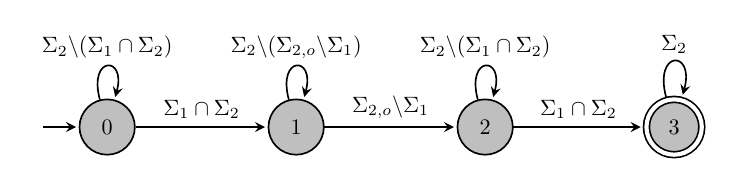
\begin{tikzpicture}
[->,>=stealth, node distance=30mm, auto, initial text=, shorten >=1pt,
semithick, 
every state/.style={fill=lightgray},
every node/.style={scale=0.8}, 
accepting/.style={double distance=1.5pt, outer sep=0.75pt+\pgflinewidth}
]
  \node[initial,state] (0)              {$0$};
  \node[state]         (1) [right of=0] {$1$};
  \node[state]         (2) [right of=1] {$2$};
  \node[state, accepting]         (3) [right of=2] {$3$};

  \path (0) edge [loop above] node {$\Sigma_2 \backslash (\Sigma_1 \cap \Sigma_2)$} (0)
  		(0) edge              node {$\Sigma_1 \cap \Sigma_2$} (1)
  		(1) edge [loop above] node {$\Sigma_2 \backslash (\Sigma_{2,o} \backslash \Sigma_1)$} (1)
        (1) edge              node {$\Sigma_{2,o} \backslash \Sigma_1$} (2)
  		(2) edge [loop above] node {$\Sigma_2 \backslash (\Sigma_1 \cap \Sigma_2)$} (2)
        (2) edge              node {$\Sigma_1 \cap \Sigma_2$} (3)
		(3) edge [loop above] node {$\Sigma_2$} (3)
%         (2) edge [bend left]  node {$\Sigma_1 \cap \Sigma_2$} (1)
        ;
\end{tikzpicture}
\caption{Automaton for marking the language $L_2$}
\label{fig:marking_L2}
% \end{figure}
% 
% \begin{figure}[t]
% \centering
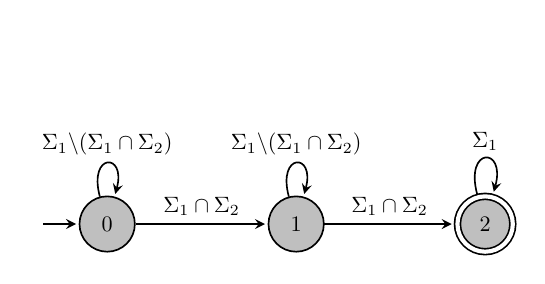
\begin{tikzpicture}
[->,>=stealth, node distance=30mm, auto, initial text=, shorten >=1pt,
semithick, 
every state/.style={fill=lightgray},
every node/.style={scale=0.8}, 
accepting/.style={double distance=1.5pt, outer sep=0.75pt+\pgflinewidth}
]
  \node[initial,state] (0)              {$0$};
  \node[] (fake) [above of=0]              {}; %for space above the picture
  \node[state]         (1) [right of=0] {$1$};
  \node[state, accepting]         (2) [right of=1] {$2$};

  \path 
	(0) edge [loop above] node {$\Sigma_1 \backslash (\Sigma_1 \cap \Sigma_2)$} (0)
	(0) edge              node {$\Sigma_1 \cap \Sigma_2$} (1)
	(1) edge [loop above] node {$\Sigma_1 \backslash (\Sigma_1 \cap \Sigma_2)$} (1)
	(1) edge              node {$\Sigma_1 \cap \Sigma_2$} (2)
	(2) edge [loop above] node {$\Sigma_1$} (2)
% 	(1) edge [bend left]  node {$\Sigma_1 \cap \Sigma_2$} (0)
    ;
\end{tikzpicture}
\caption{Automaton for marking the language $L_1$}
\label{fig:marking_L1}
\end{figure}


\subsection{Example}
Consider the system of two automata $G_1$ and $G_2$ depicted in Figure
\ref{fig:G1} and Figure \ref{fig:G2}. The set of events for the system is
$\Sigma = \{a, b, c, e, f\}$. Suppose the observable events are $\Sigma_o = \{c,
e\}$, and the set of fault events is $\{f\}$. Thus, only the language $L_1$ has a
fault, and $L_2$ has not. We use the verifier \cite{yoo_polynomial-time_2002} to
check if a language is diagnosable. The verifier for the language $L_1$ is
depicted in the Figure \ref{fig:verifier_G1}. One can check that it has an
indeterminate cycle.
The strings $fbc^*$ and $ac^*$ are not distinguishable in the local language
$L_1$. Hence, $L_1$ is not locally diagnosable.

We now use the verification procedure described in this paper to check if the
language $L_2$ can changes observation of either strings $fbc^*$ or
$ac^*$ in the language $L_1 \parallel L_2$ such that the strings become
distinguishable. The set of events common for $L_1$ and $L_2$ is $\{b, c\}$. It
can be verified that only the strings $fbc^*$ are marked by the automaton
depicted in the Figure \ref{fig:marking_L1}. Next, it can be verified that all
the strings of $L_2$ which have events common with the strings $fbc^*$ are
accepted by the automaton depicted in the Figure \ref{fig:marking_L2}. Thus, we
conclude that $L_2$ changes observation of the strings $fbc^*$ in the virtual
module $G$ built of modules $G_1$ and $G_2$, such that $G$ becomes diagnosable.
Indeed, if we make a parallel composition of the modules and build a verifier
for the result as it is depicted in the Figure \ref{fig:verifier_G1G2}, it can
be checked that the verifier has no indeterminate cycles.

\begin{figure}[t]
\centering
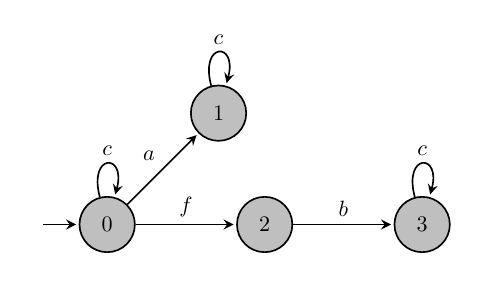
\begin{tikzpicture}
[->,>=stealth, node distance=25mm, auto, initial text=, shorten >=1pt,
semithick, 
every state/.style={fill=lightgray},
every node/.style={scale=0.8}, 
accepting/.style={double distance=1.5pt, outer sep=0.75pt+\pgflinewidth}
]
  \node[initial,state]		(0)              		{$0$};
  \node[state ]   (1) [above right of=0]	{$1$};
  \node[state]         		(2) [right of=0]		{$2$};
  \node[state]	(3) [right of=2]		{$3$};

  \path
 	(0) edge [loop above] node {$c$} (0)
 	(0) edge              node {$a$} (1)
 	(1) edge [loop above] node {$c$} (1)
 	(0) edge              node {$f$} (2)
 	(2) edge              node {$b$} (3)
 	(3) edge [loop above] node {$c$} (3)
    ;
\end{tikzpicture}
\caption{Automaton $G_1$}
\label{fig:G1}
% \end{figure}
% 
% \begin{figure}[t]
% \centering
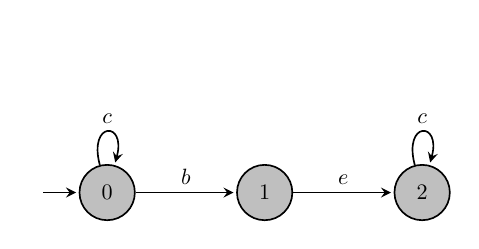
\begin{tikzpicture}
[->,>=stealth, node distance=25mm, auto, initial text=, shorten >=1pt,
semithick, 
every state/.style={fill=lightgray},
every node/.style={scale=0.8}, 
accepting/.style={double distance=1.5pt, outer sep=0.75pt+\pgflinewidth}
]
  \node[initial,state]		(0)              		{$0$};
  \node[] (fake) [above of=0] {}; %for space above the picture
  \node[state]         		(1) [right of=0]		{$1$};
  \node[state]	(2) [right of=1]		{$2$};

  \path
%  	(0) edge              node {$a$} (1)
 	(0) edge [loop above] node {$c$} (0)
 	(0) edge              node {$b$} (1)
 	(1) edge              node {$e$} (2)
 	(2) edge [loop above] node {$c$} (2)
    ;
\end{tikzpicture}
\caption{Automaton $G_2$}
\label{fig:G2}
\end{figure}

\begin{figure}[H]
\centering
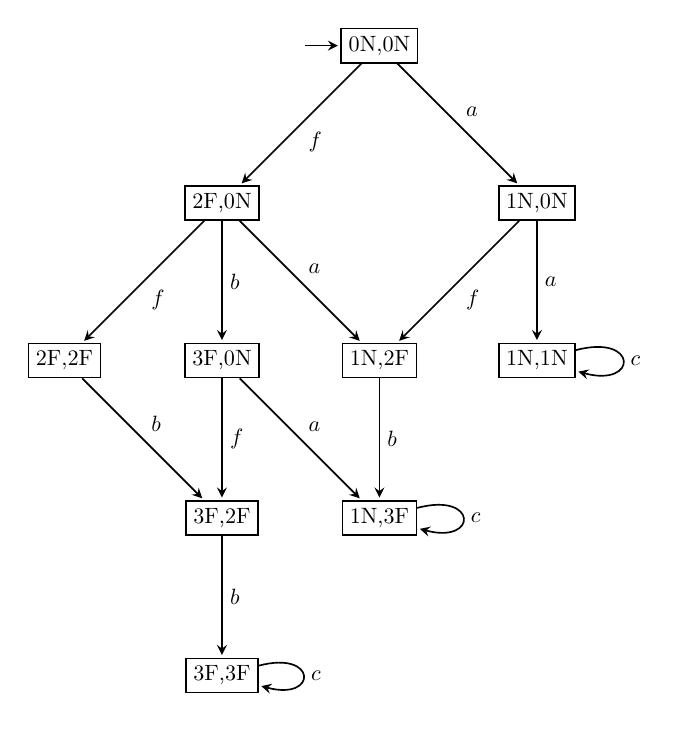
\begin{tikzpicture}
[->,>=stealth, node distance=25mm, auto, initial text=, shorten >=1pt,
semithick,
every state/.style={fill=lightgray},
every node/.style={scale=0.8},
accepting/.style={double distance=1.5pt, outer sep=0.75pt+\pgflinewidth}
]
  \node[initial,draw]		(0N0N)             			{0N,0N};
  \coordinate[below of=0N0N](fake);
  \node[draw]         		(2F0N) [left of=fake]		{2F,0N};
  \node[draw]         		(1N0N) [right of=fake]		{1N,0N};
  \node[draw]         		(3F0N) [below of=2F0N]		{3F,0N};
  \node[draw]         		(2F2F) [left of=3F0N]		{2F,2F};
  \node[draw]         		(1N2F) [right of=3F0N]		{1N,2F};
  \node[draw]         		(1N1N) [right of=1N2F]		{1N,1N};
  \node[draw]         		(3F2F) [below of=3F0N]		{3F,2F};
  \node[draw]         		(1N3F) [below of=1N2F]		{1N,3F};
  \node[draw]         		(3F3F) [below of=3F2F]		{3F,3F};

  \path
  	(0N0N) edge              node {$f$} (2F0N)
  	(0N0N) edge              node {$a$} (1N0N)
  	(2F0N) edge              node {$f$} (2F2F)
  	(2F0N) edge              node {$b$} (3F0N)
  	(2F0N) edge              node {$a$} (1N2F)
  	(1N0N) edge              node {$f$} (1N2F)
  	(1N0N) edge              node {$a$} (1N1N)
 	(1N1N) edge [loop right] node {$c$} (1N1N)
  	(2F2F) edge              node {$b$} (3F2F)
  	(3F0N) edge              node {$f$} (3F2F)
  	(3F0N) edge              node {$a$} (1N3F)
  	(1N2F) edge              node {$b$} (1N3F)
  	(1N3F) edge [loop right] node {$c$} (1N3F)
  	(3F2F) edge              node {$b$} (3F3F)
  	(3F3F) edge [loop right] node {$c$} (3F3F)
    ;
\end{tikzpicture}
\caption{Verifier of $G_1}
\label{fig:verifier_G1}
\end{figure}

\begin{figure}[t]
\centering
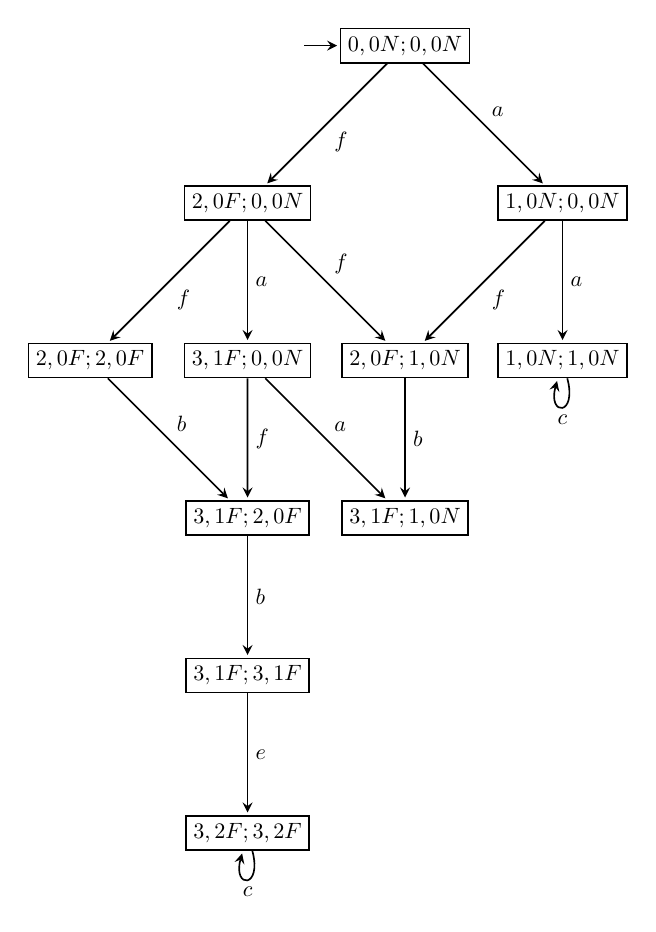
\begin{tikzpicture}
[->,>=stealth, node distance=25mm, auto, initial text=, shorten >=1pt,
semithick,
every state/.style={fill=lightgray},
every node/.style={scale=0.8}, 
accepting/.style={double distance=1.5pt, outer sep=0.75pt+\pgflinewidth}
]
  \node[draw, initial](00N00N)              	  {$0,0N;0,0N$};
  \coordinate[below of=00N00N](fake);
  \node[draw]         (20F00N) [left of =fake] {$2,0F;0,0N$};
  \node[draw]         (10N00N) [right of =fake] {$1,0N;0,0N$};
  \node[draw]         (31F00N) [below of =20F00N] {$3,1F;0,0N$};
  \node[draw]         (20F20F) [left of =31F00N]  {$2,0F;2,0F$};
  \node[draw]         (20F10N) [right of =31F00N] {$2,0F;1,0N$};
  \node[draw]         (10N10N) [right of =20F10N] {$1,0N;1,0N$};
  \node[draw]         (31F20F) [below of =31F00N] {$3,1F;2,0F$};
  \node[draw]         (31F10N) [below of =20F10N] {$3,1F;1,0N$};
  \node[draw]         (31F31F) [below of =31F20F] {$3,1F;3,1F$};
  \node[draw]         (32F32F) [below of =31F31F] {$3,2F;3,2F$};

  \path
	(00N00N) edge	node {$f$} (20F00N)
	(00N00N) edge	node {$a$} (10N00N)
	(20F00N) edge	node {$f$} (20F20F)
	(20F00N) edge	node {$f$} (20F10N)
	(20F00N) edge	node {$a$} (31F00N)
	(10N00N) edge	node {$f$} (20F10N)
	(10N00N) edge	node {$a$} (10N10N)
	(10N10N) edge [loop below] node {$c$} (10N10N)
	(20F20F) edge	node {$b$} (31F20F)
	(31F00N) edge	node {$f$} (31F20F)
	(31F00N) edge	node {$a$} (31F10N)
	(20F10N) edge	node {$b$} (31F10N)
	(31F20F) edge	node {$b$} (31F31F)
	(31F31F) edge	node {$e$} (32F32F)
	(32F32F) edge [loop below] node {$c$} (32F32F)
    ;
\end{tikzpicture}
\caption{Verifier of $G_1 \parallel G_2$}
\label{fig:verifier_G1G2}
\end{figure}


\section{Generalization. Conditions for diagnosability}

We rewrite Lemma \ref{lem:distinguished_for_2}, where the statements hold for a
system of two languages, for an arbitrary couple of languages as follows.

\begin{lemma}
\label{lem:distinguished}
Given a tuple $\left< L_i, L_j, s, u\right> \mid i, j \in \mathbb{N}, i\neq j$
and $s, u \in L_i$. The strings $s, u$ are
distinguished in the language $L_i \parallel L_j$ if for the string $s$ it
exists an adjacent observable support $K_j \subseteq L_j$ which satisfies the
condition:
\end{lemma} 
\begin{equation}
\label{con:distinquished}
	\begin{array}{l}
	 	(\forall t \in K_j)
	 	(\exists \sigma \in t \mid \sigma \in \Sigma_i \cap \Sigma_j)
	 	(\sigma \not \in u)
	 	\\
	 	(\forall w\sigma \in \overline{t})
	 	[M_j(t / w\sigma) \neq \emptyset].
	\end{array}
\end{equation}
% where $M'_j: (\Sigma_i \cup \Sigma_j)^* \rightarrow (\Sigma_{j,o}\backslash
% \Sigma_i)^*$.
Informally, the lemma imposes a requirement for the string $s$ to have an
\emph{observable support} (subset of observable strings ending with common
events) in another language, which guaranties that we can observe some events in that
language before any continuation of the string $s$.
Then, the lemma defines a condition which allows us to distinguish these
observations from the observation of the string $u$.

Now, we rewrite Lemma \ref{lem:diagnosable}, in the context of our setup, as
follows:
\begin{lemma}
\label{lem:virtual_module_is_diagnosable}
Given a virtual module $j \in J$, the module is diagnosable with respect to
$M_j$ if:
\end{lemma}
\begin{equation}
	\begin{array}{l}
% 		(\forall i \in j, s \in L_{i,f}, t \in L_i \backslash \overline{L_{i,f}})
		(\forall i \in j, 
			s \in P_i^{-1}(L_{i,f}), 
			t \in P_i^{-1}(L_{i,nf}))
% 			t \in P_i^{-1}(L_i) \backslash \overline{P_i^{-1}(L_{i,f})})
		\\
		(\exists k \in j \mid k \neq i) \textrm{ and }
		\\
		\textrm{condition (\ref{con:distinquished}) holds for at least one of
		the tuples:}
		\\
		\left<P_i^{-1}(L_i), L_k, s, t \right>,
		\left<P_i^{-1}(L_i), L_k, t, s \right>.
	\end{array}
\end{equation}
The lemma implies, that the virtual module is diagnosable if we can distinguish
all faulty strings from all non-faulty strings. 
% excluding all prefixies of the faulty strings
% Note, that exclusion of the prefixes comes from fact that the non-compositional
% analysis is used.
From the lemma it can be seen that for one faulty sublanguage there can be a
subset of languages with observable supports (a few $k\in j$), satisfying the
conditions.
In order to make the system modularly diagnosable, thus, one needs to find a
relevant partition, with a desired distribution of modules over the partition.
It worth to note, that the partitioning implies that languages with faults are
in subsets with the languages which have observable events. Thus, other
languages which have no faults and have no observable events, as well the
languages with observations which have no effect for the diagnosability
property, will be in other subsets.

One faulty module may require a few modules with observable supports.
The algorithms presented in the following section are aimed to find such subset
of system's modules. The first algorithm may be viewed as a \emph{forward
propagation} procedure. It starts from the faulty module, and propagates faulty
and non-faulty information trough all the modules, according to some
of requirements of the lemmas \ref{lem:distinguished} and
\ref{lem:virtual_module_is_diagnosable} related to common events. The second
algorithm may be viewed as a \emph{backward propagation} procedure. It starts
from a module with observable support, and propagates information related to
observable events toward the faulty module, according to the rest of the lemmas'
requirements.


\section{Inference Diagram}

The \emph{inference diagram} is a graph which reflects the structure of a
system.
The nodes of the graph are corresponded to the system's modules, the edges show that
a property of one module either is inferred by others or is inferring
properties of others. For the most of cases, the nodes are linked with edges if
the event sets of corresponding modules have common events.   

The notion of inference diagram is similar to the \emph{interaction graph} in
\cite{fabre_distributed_2005} and to the \emph{network graph} in
\cite{su_global_2005} (though it is not defined formally there).

The inference diagram is defined over the set of languages as
follows:
\begin{definition}
Given a set $S := \{L_i\mid i\in \mathbb{N}\}$. We define a binary relation
$R(S)$ for each pair $L_i, L_j \in S$ as following:
\begin{equation}
	\left<L_i, L_j \right> \in R(S) \Rightarrow 
	\Sigma_i \cap \Sigma_j \neq \emptyset.
\end{equation}
\end{definition}

For any $L_i, L_j, L_k \in S$ the relation
$R$ is:
\begin{enumerate}
  \item Reflexive: $\left<L_i, L_i \right> \in R$.
  \item Symmetric: $\left<L_i, L_j \right> \in R \Leftrightarrow 
  		\left<L_j,L_i \right> \in R$.
  \item Non-transitive: 
  		$\{\left<L_i, L_j \right>, \left<L_j, L_k \right>\} \in R
  		\not \Rightarrow \left<L_i, L_k \right> \in R$.  
\end{enumerate}

The inference diagram is used implicitly in the algorithms in the next section.
Besides its mathematical meaning the diagram has a representative value during
systems design process. An example of inference diagram for a part of the
system, presented on the Figure \ref{fig:pi_diagram}, is depicted in the Figure
\ref{fig:id_example}. It shows how models of the system modules are related to
each other. Particularly, the valve $V4$ consists of models of sensors,
actuator, the physical valve and some constraints, such that all the
corresponding nodes are linked. The nodes of the graph, corresponding to
the fork sensors $LT3$ and $LT4$ are not linked to others. However, when a model
of the control cycle will be added, these nodes become connected, reflecting
the corresponding dependencies.

\begin{figure}[!ht]
	\centering
	\includegraphics[scale=0.7]{id_example.pdf}
	\caption{Example of Inference Diagram}
	\label{fig:id_example}
\end{figure}



\section{Algorithms for diagnosability verification with virtual modules}
\label{sec:algorithms}

Assume that a language with a faulty behaviour and a language which has an
observable support are given. Then, it's required to verify if the observable
support is either for the faulty or non-faulty sublanguages. If it is true, then the
corresponding modules can be composed into a virtual module.
According to the Lemma \ref{lem:virtual_module_is_diagnosable}, in order to
decide if the virtual module is diagnosable we need to verify the necessary
conditions for all the strings $P_i^{-1}(L_{i,f})$ and $P_i^{-1}(L_{i,nf})$,
projected to the local languages of other modules $\{j \in I\mid j \neq i\}$.
Those local projections are the basic elements our algorithms operate with. In the sequel we
refer to the corresponding local sublanguages as to \emph{co-faulty} and
\emph{co-non-faulty} ones. A formal definition of these sublanguages is
presented below, and then an algorithm which computes the co-faulty
and co-non-faulty sublanguages for all the system's modules, is given. 
% It is
% followed by algorithms which verify diagnosability and find a virtual module.

\subsection{Co-faulty and co-non-faulty sublanguages}

\begin{definition}
\label{def:co-faulty}
Given $i, j \in I$, $L_{i,f} \subseteq L_i$,
we say that a sublanguage $L_{j,cf} \subseteq L_j$ is \emph{co-faulty} with
respect to $L_{i,f}$ if 
$$
	(\forall s \in L_{j,cf})(\forall t \in P_i[P_j^{-1}(s)])
	\left[
		t \in L_{i,f} \land t \not \in L_{i,nf}   
	\right],
$$ 
and a sublanguage $L_{j,cnf} \subseteq L_j$ is
\emph{co-non-faulty} with respect to $L_{i,nf}$ if 
$$
	(\forall s \in L_{j,cnf})(\forall t \in P_i[P_j^{-1}(s)])
	\left[
		t \not \in L_{i,f} \land t \in L_{i,nf}   
	\right].
$$ 
\end{definition}

In words, the co-faulty sublanguage is a sublanguage which satisfies two
conditions:
a) it is the sublanguage of projection of the global faulty language
to the local language; b) the sublanguage is not co-non-faulty.
Similarly, the co-non-faulty sublanguage is a sublanguage which satisfies
conditions:
a) it is the sublanguage of projection of the global non-faulty language
to the local language; b) the sublanguage is not co-faulty.

% \begin{lemma}
% \label{lem:empty_co_if_no_common}  
% Given a language $L_j\mid j \in I$, its co-faulty and
% co-non-faulty sublanguages are empty, if the language has no common events in
% its strings, i.e
% $$P_{\Sigma_j \rightarrow \bigcap_{i\neq j}^I \Sigma_i}(L_i) = \emptyset.$$
% \end{lemma}
% We skip the proof due to its triviality. 

Given global faulty and non-faulty sublanguages, one can compute the local
co-faulty sublanguage, using the global language, as follows:
\begin{equation}
\label{eq:co-faulty_from_global}
	\begin{array}{l}
		L_{j,cf} := P_j(L_f) \backslash P_j(L_{nf}),\\ 
		L_{j,cnf} := P_j(L_{nf}) \backslash P_j(L_{f}).	
	\end{array}
\end{equation}
However, we are interested to compute local sub languages without computing the
global language. Since the global faulty sublanguage is define as
\begin{equation}
\label{eq:co-faulty_from_locals}
	L_f := P_i^{-1}(L_{i,f}) \cap \bigcap_{k\neq
	i}^I P_k^{-1}(L_k),
\end{equation}
then, by substituting the global language in \ref{eq:co-faulty_from_global} by
\ref{eq:co-faulty_from_locals}, and by mathematical induction, the co-faulty
sublanguage of an arbitrary module can be computed as follows:

\begin{equation}
\label{eq:co-faulty_iterative_w_faulty}
	\begin{array}{l}
		L_{j,cf} := 
		\\
		P_j\Big(P_j^{-1}(L_j) \cap P_i^{-1}(L_{i,f})\cap 
		\bigcap_k^I P_k^{-1}(L_{k,cf})\Big) \backslash 
		\\
		P_j\Big(P_j^{-1}(L_j) \cap P_i^{-1}(L_{i,nf})\cap 
		\bigcap_k^I P_k^{-1}(L_{k,cnf})\Big),
		\\ 
		\textrm{where } i\neq j\neq k \in I.
	\end{array}
\end{equation}

We skip the definition of co-non-faulty sublanguage here due to its similarity. 


\subsection{Fault propagation algorithm}

\begin{alg}[!ht]
\caption{Forward propagation of a fault. Computes co-faulty and
co-non-faulty languages of all the modules}
\begin{algorithmic}[1]
	\Require The set of the system's languages $\{L_j\mid j \in I\}$, faulty and
	non-faulty sublanguages $L_{i,f}$, $L_{i,nf}$ of a faulty module $i\in I$.
	\ForAll{$j \in I$}
	\label{alg:fcf_init}
		\Comment{Initialization}
		\State $\Sigma_{j,c} \leftarrow \Sigma_j \cap \bigcup_{i\neq j}^I\Sigma_i$
		\State $C_j \leftarrow P_{j,c}(L_j)$
		\State $F_j \leftarrow \emptyset, N_j \leftarrow \emptyset$
	\EndFor
	\Procedure{propagate-fn}{$k$, $F_k$, $N_k$}
		\ForAll{$j \in I \mid j\neq k, \Sigma_j \cap \Sigma_k \neq \emptyset,
				\Sigma_{j,c}\neq \emptyset$} 
			\State $F'_j \leftarrow P_{j,c}(F_k \parallel C_j)$
			\label{alg:fcf_partial_begin}
			\State $N'_j \leftarrow P_{j,c}(N_k \parallel C_j)$ 
			\State $K \leftarrow \overline{F'_j \cap N'_j}$
			\State $F'_j \leftarrow F'_j \backslash K$
			\State $N'_j \leftarrow N'_j \backslash K$
			\label{alg:fcf_partial_end}
			\If{$F'_j \backslash F_j \neq \emptyset \lor 
				 N'_j \backslash N_j \neq \emptyset$}
				\label{alg:fcf_update}
				\State $F_j \leftarrow F_j \cup F'_j$
				\State $N_j \leftarrow N_j \cup N'_j$
				\State $\Sigma_{j,c} \leftarrow
					\{\sigma \in s \}$, where
				\State $s \in
						\left[(\overline{F_j} \backslash F_j) \cup
						(\overline{N_j} \backslash N_j)\right] \backslash	
						(\overline{F_j} \cap \overline{N_j})
						$
				\State \textproc{propagate-fn}$(j, F_j, N_j)$
			\EndIf
		\EndFor
	\EndProcedure
	
	\State $F_i \leftarrow P_{i,c}(L_{i,f})$
		\label{alg:fcf_Fi}
	\State $N_i \leftarrow P_{i,c}(L_{i,nf})$
	\State \textproc{propagate-fn}($i$, $F_i$, $N_i$)
	\Comment{Beginning of recursion}	
	\ForAll{$j \in I \mid j \neq i$}
		\Comment{Finalization}
		\label{alg:fcf_final}
		\State $L_{j,cf} \leftarrow L_j \cap P_{j,c}^{-1}(F_j)$
		\State $L_{j,cnf} \leftarrow L_j \cap P_{j,c}^{-1}(N_j)$
	\EndFor
	\\
	\Return $\{L_{j,cf}\}$, $\{L_{j,cnf}\}$
\end{algorithmic}
\label{alg:propagate_fn}
\end{alg}


Now, we present Algorithm \ref{alg:propagate_fn} which, given a module with a
faulty behaviour defined, computes the co-faulty and co-non-faulty languages for
all the rest modules of the system.
The algorithm starts from a preliminary step at line \ref{alg:fcf_init}.
At this step a projection to the common events $C_j$ is computed for all the
local languages. Projections of co-faulty and co-non-faulty sublanguages to the
common events, denoted as $F_j, N_j$, are empty in the beginning. Event sets
$\Sigma_{j,c}$ are sets of the common events, which don't belong neither to
co-faulty and co-non-faulty sublanguages nor to intersection of the
sublanguages' prefix-closures. Since that sublanguages are not defined in the
beginning, the event sets contain all events from the projections. A role of
these sets will be clarified later.
The recursive procedure \emph{propagate-fn} computes $F_j$ and $N_j$ for all the
system's modules, except the module with a fault; the procedure operates with
common events only. Before entering the procedure the projections of the faulty
module's sublanguages, $F_i, N_i$ are computed at the step \ref{alg:fcf_Fi}.
Note, that projection operation preserves faulty and non-faulty information,
when faulty behaviour is defined in a specification-based way.

The recursive procedure computes all projections $F_j, N_j$ of the modules
adjacent to a given module $k$ (we say that two modules are adjacent to each
other if their languages have events in common). At the first steps
\ref{alg:fcf_partial_begin}-\ref{alg:fcf_partial_end} of the procedure we
compute $F'_j, N'_j$ with respect to the module $k$; these projections are
partial. The parallel composition $F_k \parallel C_j$, followed by projection to
the common events, is used to extract the faulty information from the
language $F_k$ to $C_j$, and non-faulty from $N_k$ to $C_j$. At the step
\ref{alg:fcf_update} we check if some co-faulty or co-non-faulty strings should be added to the projections computed earlier. If so, then we update $F_j, N_j$, $\Sigma_{j,c}$ and call the same procedure to update projections of the adjacent modules. Thus, whenever the co-faulty or
co-non-faulty projections of that module changed, the projections $F_j, N_j$ are
updating with respect to every other module, due to recursion. The event sets
$\Sigma_{j,c}$ represent a potentiality that the projections $F_j, N_j$ can be
changed; the modules which have these sets empty can't change their language's
property with respect to the fault and, thus, are skipped during recursive
procedure. Finally, all the co-faulty and co-non-faulty sublanguages are
calculated for each module at the step \ref{alg:fcf_final}.



%%%%%%%%%%%%%%%%%%%%%%%%%%%%%%%%%%%%%%%%%%%%%%%%%%%%%%%%%%%%%%%%%%%%%%%%%%%%%%%
\subsection{Observation propagation algorithm}

\begin{alg} 
\caption{Backward propagation of the fault observation. Computes observable
information for the faulty module} 
\begin{algorithmic}[1]
	\Require The index  $i \in I$ of the faulty module, the index of a module with
	observable support $k \in I \mid M(L_{k,cf}) \neq \emptyset \lor M(L_{k,cnf})
	\neq \emptyset, k \neq i$, the sets $\{L_{j,cf}\}, \{L_{j,cnf}\}, j \in I$.
% 	\State $V \leftarrow \{i\}$ \Comment{Virtual module}

	\ForAll{$j \in I$}
	\label{alg:fco_init}
		\State $D_{j,f} \leftarrow P_{j,co}(L_{j,f})$
		\State $D_{j,nf} \leftarrow P_{j,co}(L_{j,nf})$
	\EndFor
	
	\Procedure{propagate-d}{$k$, $D_{k,f}$, $D_{k,nf}$}
		\ForAll{$j \in I \mid \Sigma_j \cap \Sigma_k \neq \emptyset$}
			\State $D'_{j,f} \leftarrow 
			P_{j,co}(F_j \parallel D_{k,f})$
			\If{$(D'_{j,f}\backslash D_{j,f} \neq \emptyset) \lor
				(D'_{j,nf}\backslash D_{j,nf} \neq \emptyset)$}
				\State $D_{j,f}\leftarrow D'_{j,f}$
				\State $D_{j,nf}\leftarrow D'_{j,nf}$
				\State \textproc{propagate-d}($j$, $D_{j,f}$, $D_{j,nf}$)
			\EndIf
		\EndFor 
	\EndProcedure
	
	\State \textproc{propagate-d}($k$, $D_{k,f}$, $D_{k,nf}$)
	\label{alg:fco_enter_recursion}
	\State $L_{i,f}^{ext} \leftarrow P_{i,co}(L_{i,f} \parallel D_{i,f})$
	\label{alg:fco_finalize}
	\State $L_{i,nf}^{ext} \leftarrow P_{i,co}(L_{i,nf} \parallel D_{i,nf})$
	\\
	\Return $L_{i,f}^{ext}, L_{i,nf}^{ext}$
\end{algorithmic}
\label{alg:propagate-d}
\end{alg}

The structure of the Algorithm \ref{alg:propagate-d} is similar to one
in Algorithm \ref{alg:propagate_fn}. It starts from computing projections to
common and observable events for the co-faulty and co-non-faulty sublanguages of each
module's language. Then, starting from the module $k$ which has observable
events in its sublanguages (i.e. it has potential observable support for a
sublanguage of the faulty module), begins a recursive procedure at step
\ref{alg:fco_enter_recursion}.
In the procedure we collect only observable events of other modules which are related to co-faulty or co-non-faulty
sublanguages. Then we propagated these events down to the faulty module.
Finally, at the step \ref{alg:fco_finalize}, the faulty and non-faulty
sublanguages of the faulty module are extended with observable events.

The result of the Algorithm \ref{alg:propagate-d}, the faulty and non-faulty
sublanguages extended with observable events, can be used to verify
diagnosability now. Any approach, which allows us to check for the presence of
indistinguishable strings in the language (the faulty and non-faulty
sublanguages can be united, if necessary), is suitable. We can have the
following outcomes after verification: a) no indistinguishable strings are
broken, b) no indistinguishable strings left, and c) some indistinguishable
strings are broken. In case (a) we pick another module $k \in I$ satisfying
requirements of the Algorithm \ref{alg:propagate-d} for further processing and
verification. In case (b) we may construct a virtual module of the faulty module
$i$ and the module $k$ and declare that the fault is diagnosable with respect to
the virtual module $\{i, k\}$ and stop, or continue and check if it exists
another module which can also be used to build a virtual module. In case (c) we should
pick additional module satisfying requirements of the Algorithm
\ref{alg:propagate-d} and continue the process until all the indistinguishable
strings are broken. The following section analyzes what may be considered as a
criteria for choosing the module with observable support $k$.


\subsection{Algorithm to choose a module with observable support}
Assume that the objective function is to have the number of modules in the
system as many as possible, i.e. to have the maximal cardinality of the
partition $J$.
Given an initial set of languages, let rank of $J$ be equal to 0, i.e. $|J| =
|I|$. Let $F$ denotes the subset of languages with faults, and $M$ denotes the
subset of languages with corresponding observable supports.
Assume that it is always possible to make the system modularly diagnosable with
respect to some virtual modules. Then we know that $(\forall f \in F)~\exists m
\in M$. Let $F \cap M = \emptyset$ and $|M| \geq |F|$. Then, to make the system
modularly diagnosable it is required, in the worst case, $|F|$ members of $M$.
Thus, the cardinality of the systems with virtual modules, i.e. the cardinality
of the partition, in the worst case is:
\begin{equation}
	\min |J| = |I| - |F|.
\end{equation}
Let $M \subseteq F$. Then, the cardinality of the partition in the best case
is:
\begin{equation}
	\max |J| = |I| - \left(
		\left\lfloor \frac{|F|}{2} \right\rfloor + \textrm{mod} \frac{|F|}{2}
		\right). 
\end{equation}

As can be seen from the above, in order to maximize the number of modules while
making the virtual modules, we should consider, firstly, the modules which
themselves have faults. We propose a procedure for the given objective function
as follows:

Given the system of cardinality $|I|$, the subset $F \subseteq I$ of modules
with faults, such that any $f\in F$ is not diagnosable locally, the subset $M
\subseteq I$ of modules with observable supports, such that $(\forall f \in
F)~\{m \in M\}\neq \emptyset$. In order to make the system diagnosable by
the minimal number of virtual modules:
\begin{enumerate}
  \item Initially set the partition $J$ of $I$ such that the rank of $J$ is
  equal to 0;
  \item $(\forall j \in J, f \in j)$ update $j$ as follows: 
  	$j := j \cup \{m \in M \cap F\}$ if $M \cap F \neq \emptyset$,
 $j := j \cup \{m \in M\}$ otherwise, where $\{m\}$ is a singleton of the
 arbitrary chosen observable support for the given $f$, such that the new $j$
 is locally diagnosable; exclude $m$ from $k \in J \mid k \neq j$, and remove
 $k$ from $J$ if $k=\emptyset$.
\end{enumerate} 
The order the observable supports are verified in the procedure guaranties that
we consider the languages which themselves contain the faulty
sublanguages at first, thus maximizing the number of virtual modules in the
system.

It worth to note that the above algorithm can be augmented by additional
criteria aimed, for instance, to decrease computational burden.


%%%%%%%%%%%%%%%%%%%%%%%%%%%%%%%%%%%%%%%%%%%%%%%%%%%%%%%%%%%%%%%%%%%%%%%%%%%%%%%
\section{Example}
\label{sec:Example}
An example with languages presented by automata (see the Figures \ref{fig:G1-4}
-- \ref{fig:L1_extended}) shows how the algorithms \ref{alg:propagate_fn} and
\ref{alg:propagate-d} can be applied to a simple system. We use marked states to
mark strings in languages, since they are not prefix-closed, in general. The
system consists of three modules as depicted in Figure \ref{fig:G1-4}. Here a
fault is presented only in the language $L_1$ by the event $f$.
Figure \ref{fig:G1_faulty} depicts faulty and non-faulty sublanguages of the
language $L_1$. Projections of these sublanguages to the common events (step
\ref{alg:fcf_Fi} of the Algorithm \ref{alg:propagate_fn}), $F_1$ and $N_1$ are
depicted in the Figure \ref{fig:FN}. Suppose that in the beginning of the
recursive procedure we pick module $2$. The figure depicts the co-faulty
and co-non-faulty sublanguage of the language $L_2$ with respect to the language
$L_1$, calculated at the steps \ref{alg:fcf_partial_begin} of the algorithm (we
don't show intermediate automata, reflecting compositional steps, due to space
restrictions). Note, that, when calculated, the event set $\Sigma_{2,c}$ is
empty for module $2$. Hence this module will not participate in the procedure
as a module adjacent to others. At the next step we randomly pick the language
$L_4$, and compute $F_4$ and $N_4$ with respect to the module $2$. Now, note
that $\Sigma_{3,c}:= \{e\}$, since this event is neither in the co-faulty and
co-non-faulty projections nor in their common prefix. The iterations is followed
by the module $3$, which has module $4$ as an adjacent one. Therefore, the
sublanguages of this module are updated.

Figure \ref{fig:L4_f} depicts co-faulty and co-non-faulty sublanguages of module
$4$ calculated at the step \ref{alg:fco_finalize} of the Algorithm
\ref{alg:propagate_fn}. It shows that the co-faulty sublanguage of the module
has an observable support; it satisfies the requirements of the Lemma
\ref{lem:distinguished}. Other modules with no faults have no observable
events; they have no observable supports, and not depicted.

The major steps of Algorithm \ref{alg:propagate-d} are depicted in the Figure
\ref{fig:D}. It is shown how the observable information from the module $4$ is
propagated backward to the language of the module $1$. The final step of the
algorithm is depicted in the Figure \ref{fig:L1_extended}. Clearly, the faulty
and non-faulty sublanguages, extended with observable information, have
distinguished observations. Then, we can conclude that the virtual module
composed of the modules $1$ and $4$ is locally diagnosable. Hence, the system is
modularly diagnosable with modularity presented by the partition 
$\{\{1,4\}, \{2\}, \{3\}\}$.



\begin{figure}[t]
\centering
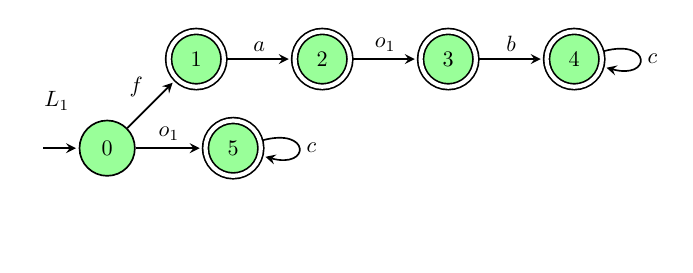
\begin{tikzpicture}[->,>=stealth, node distance=2cm, auto, shorten >=1pt,
semithick, initial text=,	
	every node/.style={scale=0.8},
    every state/.style={fill=green!40,text=black},
    accepting/.style={double distance=1.5pt, outer sep=0.75pt+\pgflinewidth}
    ]
% \draw[help lines] (0,-2) grid (6,2);
% G1
\node[initial,state] (0)                    {$0$};
\node[above left = 0.5em of 0]{$L_{1}$};
\node[state, accepting]         (1) [above right of=0] {$1$};
\node[state, accepting]         (2) [right of=1]       {$2$};
\node[state, accepting]         (3) [right of=2]       {$3$};
\node[state, accepting]         (4) [right of=3]       {$4$};
\node[state, accepting]         (5) [right of=0] 		{$5$};
\node[]         () [below right of=0] 		{}; %some blank space
\path
(0)	edge [] 		 node {$f$} (1)
(1)	edge [] 		 node {$a$} (2)
(2)	edge [] 		 node {$o_1$} (3)
(3)	edge [] 		 node {$b$} (4)
(4)	edge [loop right] node {$c$} (4)
(0)	edge [] 		 node {$o_1$} (5)
(5)	edge [loop right] node {$c$} (5)
;
\end{tikzpicture}
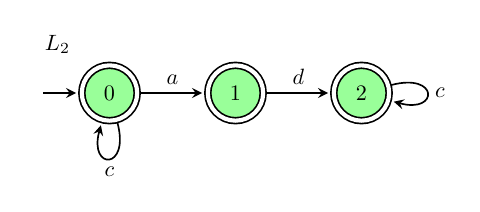
\begin{tikzpicture}[->,>=stealth, node distance=2cm, auto, shorten >=1pt,
semithick, initial text=,	
	every node/.style={scale=0.8},
    every state/.style={fill=green!40,text=black},
    accepting/.style={double distance=1.5pt, outer sep=0.75pt+\pgflinewidth}
    ]
% \draw[help lines] (0,-2) grid (6,2);
% G2
\node[initial,state, accepting] (0)                    {$0$};
\node[above left = 0.5em of 0]{$L_{2}$};
\node[state, accepting]         (1) [right of=0] 		{$1$};
\node[state, accepting]         (2) [right of=1]       {$2$};
\path
(0)	edge [] 		  node {$a$} (1)
	edge [loop below] node {$c$} (0)
(1)	edge [] 		  node {$d$} (2)
(2)	edge [loop right] node {$c$} (2)
;
\end{tikzpicture}
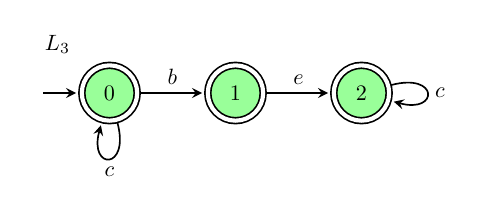
\begin{tikzpicture}[->,>=stealth, node distance=2cm, auto, shorten >=1pt,
semithick, initial text=,	
	every node/.style={scale=0.8},
    every state/.style={fill=green!40,text=black},
    accepting/.style={double distance=1.5pt, outer sep=0.75pt+\pgflinewidth}
    ]
% G3
% \node[initial,state, accepting] (0') [below of=0]      {$0$};
\node[initial,state, accepting] (0') []      {$0$};
\node[above left = 0.5em of 0']{$L_{3}$};
\node[state, accepting]         (1') [right of=0']		{$1$};
\node[state, accepting]         (2') [right of=1']     {$2$};
\path
(0')	edge [] 		  node {$b$} (1')
		edge [loop below] node {$c$} (0')
(1')	edge [] 		  node {$e$} (2')
(2')	edge [loop right] node {$c$} (2')
;
\end{tikzpicture}
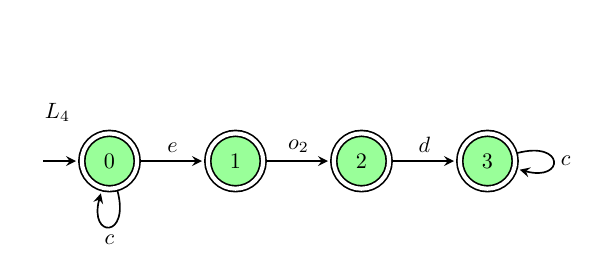
\begin{tikzpicture}[->,>=stealth, node distance=2cm, auto, shorten >=1pt,
semithick, initial text=,	
	every node/.style={scale=0.8},
    every state/.style={fill=green!40,text=black},
    accepting/.style={double distance=1.5pt, outer sep=0.75pt+\pgflinewidth}
    ]
% G4
% \node[initial,state, accepting] (0'') [below of=0']  {$0$};
\node[initial,state, accepting] (0'') []  {$0$};
\node[] (fake) [above of=0''] {}; %for space above the picture
\node[above left = 0.5em of 0'']{$L_{4}$}; 
\node[state, accepting]         (1'') [right of=0'']	{$1$};
\node[state, accepting]         (2'') [right of=1'']   {$2$};
\node[state, accepting]         (3'') [right of=2'']   {$3$};
\path
(0'')	edge [] 		  node {$e$} (1'')
		edge [loop below] node {$c$} (0'')
(1'')	edge [] 		  node {$o_2$} (2'')
(2'')	edge [] 		  node {$d$} (3'')
(3'')	edge [loop right] node {$c$} (3'')
;
\end{tikzpicture}
\caption{Automata marking languages $L_1, L_2, L_3$ and $L_4$. $\Sigma_o :=
\{o_1, o_2\}$, $\Sigma_f := \{f\}$}
\label{fig:G1-4}
\end{figure}

% Fautly and non-faulty
\begin{figure}[t]
% \centering
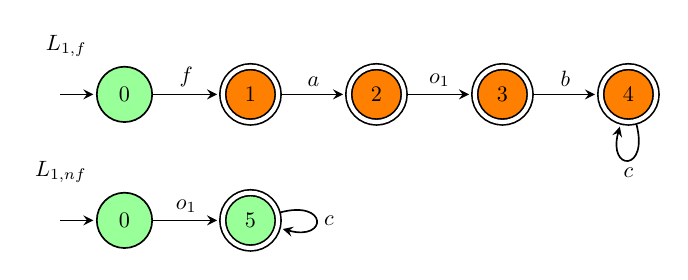
\begin{tikzpicture}[->,>=stealth, node distance=2cm, auto, shorten >=1pt,
semithick, initial text=,	
	every node/.style={scale=0.8},
    every state/.style={fill=green!40,text=black},
    accepting/.style={double distance=1.5pt, outer sep=0.75pt+\pgflinewidth}
    ]
% \draw[help lines] (0,-2) grid (6,2);
\node[initial,state] (0)                    {$0$};
% \node[above = 3em of 0] {}; %adds some space above
\node[above left = 0.5em of 0]{$L_{1,f}$};
\node[state, accepting, fill=orange]         (1) [right of=0] 		{$1$};
\node[state, accepting, fill=orange]         (2) [right of=1]       {$2$};
\node[state, accepting, fill=orange]         (3) [right of=2]       {$3$};
\node[state, accepting, fill=orange]         (4) [right of=3]       {$4$};

\node[initial,state] (0') [below of=0]                   {$0$};
\node[above left = 0.5em of 0']{$L_{1,nf}$};
\node[state, accepting]         (5)
[right of=0'] 		{$5$};

\path
(0)	edge [] 		 node {$f$} (1)
(1)	edge [] 		 node {$a$} (2)
(2)	edge [] 		 node {$o_1$} (3)
(3)	edge [] 		 node {$b$} (4)
(4)	edge [loop below] node {$c$} (4)
;
\path
(0') edge [] 		 node {$o_1$} (5)
(5)	edge [loop right] node {$c$} (5)
;
\end{tikzpicture}
\caption{Automata marking the faulty and non-faulty sublanguages of $L_1$}
\label{fig:G1_faulty}
% \end{figure}

% Projection to common events (G1)
% \begin{figure}[t!]
% \centering
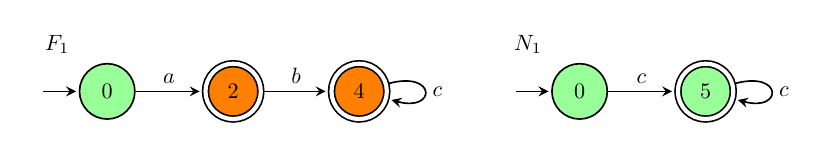
\begin{tikzpicture}[->,>=stealth, node distance=2cm, auto, shorten >=1pt,
semithick, initial text=,	
	every node/.style={scale=0.8},
    every state/.style={fill=green!40,text=black},
    accepting/.style={double distance=1.5pt, outer sep=0.75pt+\pgflinewidth}
    ]
% \draw[help lines] (0,-2) grid (6,2);
\node[initial,state] (0)                    {$0$};
% \node[above = 3em of 0] {}; %adds some space above
\node[above left = 0.5em of 0]{$F_1$};
\node[state, accepting, fill=orange]         (2) [right of=0]       {$2$};
\node[state, accepting, fill=orange]         (4) [right of=2]       {$4$};

\node[initial,state] (0') [] at (6,0)              {$0$};
\node[above left = 0.5em of 0']{$N_1$};
\node[state, accepting]         (5) [right of=0'] 		{$5$};

\path
(0)	edge [] 		 node {$a$} (2)
(2)	edge [] 		 node {$b$} (4)
(4)	edge [loop right] node {$c$} (4)
;
\path
(0') edge [] 		 node {$c$} (5)
(5)	edge [loop right] node {$c$} (5)
;
\end{tikzpicture}
\\

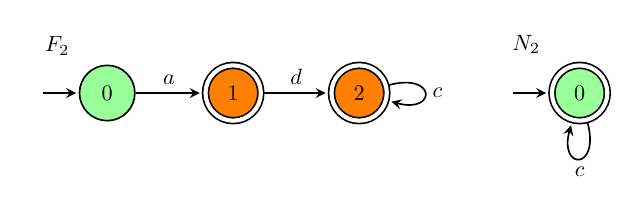
\begin{tikzpicture}[->,>=stealth, node distance=2cm, auto, shorten >=1pt,
semithick, initial text=,	
	every node/.style={scale=0.8},
    every state/.style={fill=green!40,text=black},
    accepting/.style={double distance=1.5pt, outer sep=0.75pt+\pgflinewidth}
    ]
% \draw[help lines] (0,-2) grid (6,2);
% F2
\node[initial,state] (0)                    {$0$};
\node[above left = 0.5em of 0]{$F_2$};
\node[state, accepting, fill=orange]         (1) [right of=0] 		{$1$};
\node[state, accepting, fill=orange]         (2) [right of=1]       {$2$};
\path
(0)	edge [] 		  node {$a$} (1)
(1)	edge [] 		  node {$d$} (2)
(2)	edge [loop right] node {$c$} (2)
;
% F2
\node[initial,state, accepting] (0') at (6,0) {$0$};
\node[above left = 0.5em of 0']{$N_2$};
\path
(0') edge [loop below] node {$c$} (0')
;
\end{tikzpicture}

\newline

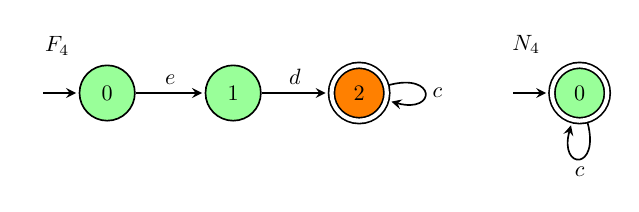
\begin{tikzpicture}[->,>=stealth, node distance=2cm, auto, shorten >=1pt,
semithick, initial text=,	
	every node/.style={scale=0.8},
    every state/.style={fill=green!40,text=black},
    accepting/.style={double distance=1.5pt, outer sep=0.75pt+\pgflinewidth}
    ]
% \draw[help lines] (0,-2) grid (6,2);
% F4
\node[initial,state] (0)                    {$0$};
\node[above left = 0.5em of 0]{$F_4$};
\node[state ]         (1) [right of=0] 		{$1$};
\node[state, accepting, fill=orange]         (2) [right of=1]       {$2$};
\path
(0)	edge [] 		  node {$e$} (1)
(1)	edge [] 		  node {$d$} (2)
(2)	edge [loop right] node {$c$} (2)
;
\node[initial,state, accepting] (0') at (6,0) {$0$};
\node[above left = 0.5em of 0']{$N_4$};
\path
(0') edge [loop below] node {$c$} (0')
;
\end{tikzpicture}

\newline

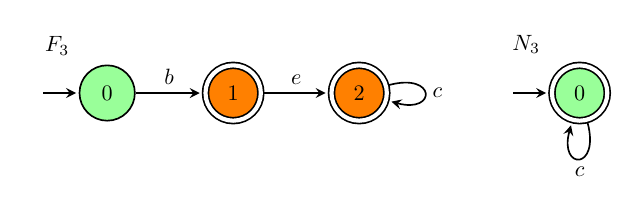
\begin{tikzpicture}[->,>=stealth, node distance=2cm, auto, shorten >=1pt,
semithick, initial text=,	
	every node/.style={scale=0.8}, 
	every state/.style={fill=green!40,text=black},
    accepting/.style={double distance=1.5pt, outer sep=0.75pt+\pgflinewidth}
    ]
% \draw[help lines] (0,-2) grid (6,2);
% F3
\node[initial,state] (0)                    {$0$};
\node[above left = 0.5em of 0]{$F_3$};
\node[state, accepting, fill=orange]         (1) [right of=0] 		{$1$};
\node[state, accepting, fill=orange]         (2) [right of=1]       {$2$};
\path
(0)	edge [] 		  node {$b$} (1)
(1)	edge [] 		  node {$e$} (2)
(2)	edge [loop right] node {$c$} (2)
;
\node[initial,state, accepting] (0') at (6,0) {$0$};
\node[above left = 0.5em of 0']{$N_3$};
\path
(0') edge [loop below] node {$c$} (0')
;
\end{tikzpicture}

\newline

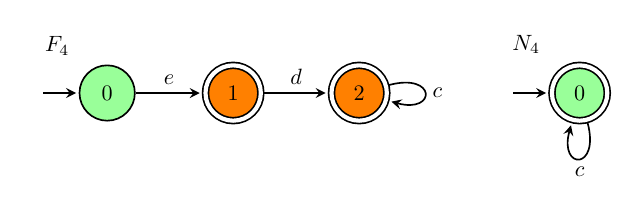
\begin{tikzpicture}[->,>=stealth, node distance=2cm, auto, shorten >=1pt,
semithick, initial text=,	
	every node/.style={scale=0.8},
    every state/.style={fill=green!40,text=black},
    accepting/.style={double distance=1.5pt, outer sep=0.75pt+\pgflinewidth}
    ]
% \draw[help lines] (0,-2) grid (6,2);
% F4
\node[initial,state] (0)                    {$0$};
\node[above left = 0.5em of 0]{$F_4$};
\node[state, accepting, fill=orange]         (1) [right of=0] 		{$1$};
\node[state, accepting, fill=orange]         (2) [right of=1]       {$2$};
\path
(0)	edge [] 		  node {$e$} (1)
(1)	edge [] 		  node {$d$} (2)
(2)	edge [loop right] node {$c$} (2)
;
\node[initial,state, accepting] (0') at (6,0) {$0$};
\node[above left = 0.5em of 0']{$N_4$};
\path
(0') edge [loop below] node {$c$} (0')
;
\end{tikzpicture}

\caption{Automata marking sublanguages $F_1$ and $N_1$ of the faulty module,
and co-faulty and co-non-faulty languages of the modules 2, 3 and 4 in the
order they are composed (top-down): 1-2, 2-4, 1-3, 3-4. Note, that the
sublanguage $F_4$ is defined partially at first, then fully}
\label{fig:FN}
\end{figure}

% Fautly and non-faulty
\begin{figure}[t]
% \centering
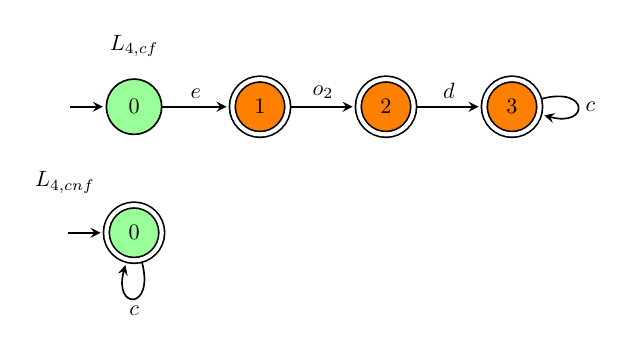
\begin{tikzpicture}[->,>=stealth, node distance=2cm, auto, shorten >=1pt,
semithick, initial text=,	
	every node/.style={scale=0.8},
    every state/.style={fill=green!40,text=black},
    accepting/.style={double distance=1.5pt, outer sep=0.75pt+\pgflinewidth}
    ]
\node[initial,state] (0) {$0$};
\node[above = 0.5em of 0]{$L_{4,cf}$}; 
\node[state, accepting, fill=orange]         (1) [right of=0]	{$1$};
\node[state, accepting, fill=orange]         (2) [right of=1]   {$2$};
\node[state, accepting, fill=orange]         (3) [right of=2]   {$3$};
\path
(0)	edge [] 		  node {$e$} (1)
(1)	edge [] 		  node {$o_2$} (2)
(2)	edge [] 		  node {$d$} (3)
(3)	edge [loop right] node {$c$} (3)
;
\node[initial,state, accepting] (0') [below of=0] {$0$};
\node[above left = 0.5em of 0']{$L_{4,cnf}$};
\path
(0') edge [loop below] node {$c$} (0')
;
\end{tikzpicture}
\caption{Automata marking co-faulty and co-non-faulty sublanguages of
the language $L_4$. Automata for the sublanguages of the modules 2 and 3 are
equal to the ones depicted in the Figure \ref{fig:FN}}
\label{fig:L4_f}
% \end{figure}

% Projections to common and observable events
% \begin{figure}[t]
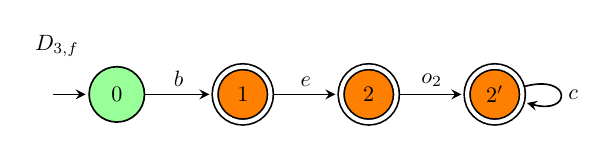
\begin{tikzpicture}[->,>=stealth, node distance=2cm, auto, shorten >=1pt,
semithick, initial text=,	
	every node/.style={scale=0.8}, 
	every state/.style={fill=green!40,text=black},
    accepting/.style={double distance=1.5pt, outer sep=0.75pt+\pgflinewidth}
    ]
% \draw[help lines] (0,-2) grid (6,2);
% F3
\node[initial,state] (0)                    {$0$};
% \node[above = 3em of 0] {}; %adds some space above
\node[above left = 0.5em of 0]{$D_{3,f}$};
\node[state, accepting, fill=orange]         (1) [right of=0] 		{$1$};
\node[state, accepting, fill=orange]         (2) [right of=1]       {$2$};
\node[state, accepting, fill=orange]         (2') [right of=2]       {$2'$};
\path
(0)	edge [] 		  node {$b$} (1)
(1)	edge [] 		  node {$e$} (2)
(2)	edge [] 		  node {$o_2$} (2')
(2')	edge [loop right] node {$c$} (2')
;
\end{tikzpicture}
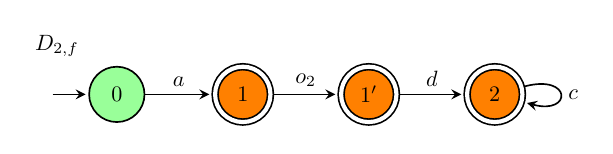
\begin{tikzpicture}[->,>=stealth, node distance=2cm, auto, shorten >=1pt,
semithick, initial text=,	
	every node/.style={scale=0.8},
    every state/.style={fill=green!40,text=black},
    accepting/.style={double distance=1.5pt, outer sep=0.75pt+\pgflinewidth}
    ]
\node[initial,state] (0)                    {$0$};
\node[above left = 0.5em of 0]{$D_{2,f}$};
\node[state, accepting, fill=orange]         (1) [right of=0] 		{$1$};
\node[state, accepting, fill=orange]         (1') [right of=1] 		{$1'$};
\node[state, accepting, fill=orange]         (2) [right of=1']       {$2$};
\path
(0)	edge [] 		  node {$a$} (1)
(1)	edge [] 		  node {$o_2$} (1')
(1')edge [] 		  node {$d$} (2)
(2)	edge [loop right] node {$c$} (2)
;
\end{tikzpicture}
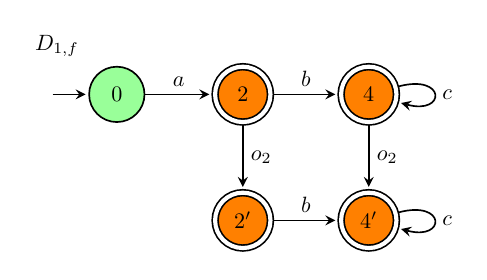
\begin{tikzpicture}[->,>=stealth, node distance=2cm, auto, shorten >=1pt,
semithick, initial text=,	
	every node/.style={scale=0.8},
    every state/.style={fill=green!40,text=black},
    accepting/.style={double distance=1.5pt, outer sep=0.75pt+\pgflinewidth}
    ]
% \draw[help lines] (0,-2) grid (6,2);
\node[initial,state] (0)                    {$0$};
\node[above left = 0.5em of 0]{$D_{1,f}$};
\node[state, accepting, fill=orange]         (2) [right of=0]       {$2$};
\node[state, accepting, fill=orange]         (2') [below of=2]      
{$2'$}; \node[state, accepting, fill=orange]         (4) [right of=2]      {$4$};
\node[state, accepting, fill=orange]         (4')[below of=4]{$4'$};
\path
(0)	edge [] 		 node {$a$} (2)
(2)	edge [] 		 node {$b$} (4)
	edge [] 		node {$o_2$} (2')
(2')edge [] 		 node {$b$} (4')
(4)	edge [loop right] node {$c$} (4)
	edge [] 		node {$o_2$} (4')
(4')edge [loop right] node {$c$} (4')
;
\end{tikzpicture}
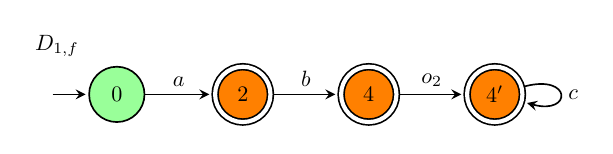
\begin{tikzpicture}[->,>=stealth, node distance=2cm, auto, shorten >=1pt,
semithick, initial text=,	
	every node/.style={scale=0.8},
    every state/.style={fill=green!40,text=black},
    accepting/.style={double distance=1.5pt, outer sep=0.75pt+\pgflinewidth}
    ]
% \draw[help lines] (0,-2) grid (6,2);
\node[initial,state] (0)                    {$0$};
\node[above left = 0.5em of 0]{$D_{1,f}$};
\node[state, accepting, fill=orange]         (2) [right of=0]       {$2$};
\node[state, accepting, fill=orange]         (4) [right of=2]       {$4$};
\node[state, accepting, fill=orange]         (4')[right of=4] {$4'$};
\path
(0)	edge [] 		 node {$a$} (2)
(2)	edge [] 		 node {$b$} (4)
(4) edge [] 		node {$o_2$} (4')
(4')edge [loop right] node {$c$} (4')
;
\end{tikzpicture}
\caption{Automata marking $D_{j,f}$ of the modules 1, 2 and 3 in
the order they are composed (top-down): 4-3, 4-2, 2-1, 3-1. Automata marking
$D_{j,nf}$ are not depicted since they have no observable events}
\label{fig:D}
% \end{figure}


% Fautly and non-faulty
% \begin{figure}[t!]
% \centering
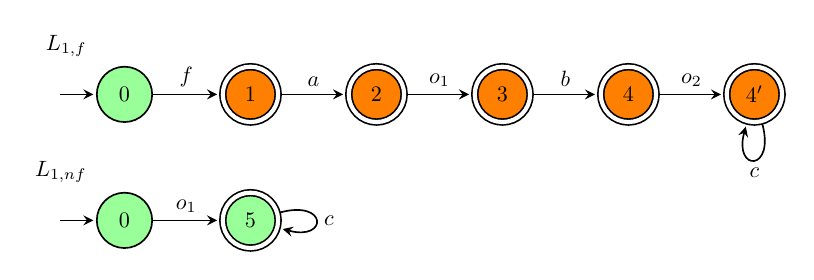
\begin{tikzpicture}[->,>=stealth, node distance=2cm, auto, shorten >=1pt,
semithick, initial text=,	
	every node/.style={scale=0.8},
    every state/.style={fill=green!40,text=black},
    accepting/.style={double distance=1.5pt, outer sep=0.75pt+\pgflinewidth}
    ]
% \draw[help lines] (0,-2) grid (6,2);
\node[initial,state] (0)                    {$0$};
% \node[above = 3em of 0] {}; %adds some space above
\node[above left = 0.5em of 0]{$L_{1,f}$};
\node[state, accepting, fill=orange]         (1) [right of=0] 		{$1$};
\node[state, accepting, fill=orange]         (2) [right of=1]       {$2$};
\node[state, accepting, fill=orange]         (3) [right of=2]       {$3$};
\node[state, accepting, fill=orange]         (4) [right of=3]       {$4$};
\node[state, accepting, fill=orange]         (4')[right of=4]       {$4'$};

\node[initial,state] (0') [below of=0]                   {$0$};
\node[above left = 0.5em of 0']{$L_{1,nf}$};
\node[state, accepting]         (5)
[right of=0'] 		{$5$};

\path
(0)	edge [] 		 node {$f$} (1)
(1)	edge [] 		 node {$a$} (2)
(2)	edge [] 		 node {$o_1$} (3)
(3)	edge [] 		 node {$b$} (4)
(4) edge [] 		 node {$o_2$} (4')
(4')edge [loop below] node {$c$} (4')

;
\path
(0') edge [] 		 node {$o_1$} (5)
(5)	edge [loop right] node {$c$} (5)
;
\end{tikzpicture}
\caption{Automata marking the faulty and non-faulty sublanguages of $L_1$ after
the backward Algorithm. The observation of $L_{1,f}$ is $\{o_1o_2\}$ differs
from the observation of $L_{1,nf}$ which is $\{o_1\}$}
\label{fig:L1_extended}
\end{figure}


\section{Related approaches}

The notion of virtual modular diagnosability was initially introduced in this
work. However, this approach can be decomposed into a few techniques, and a
few works, each solving similar problems, can be found in literature. These
studies are described in the following.

An interesting approach is developed in \cite{rudie_minimal_1999},
\cite{rudie_minimal_2003} and \cite{lin_minimal_2007} where the authors start
from the assumption that the modules of a system require communication to each
other in order to make a decision (e.g. about a failure), but the information
they exchange can be redundant. They try to minimize communications globally and
provide a solution with exponential time complexity. This approach is
completely different to the one presented in this work, since it does not change
modularity of the system. However, the idea to reduce redundant communication
may result in a higher modularity in our context.

In \cite{ye_incremental_2009} and \cite{ye_general_2012} the authors verify
distributed diagnosability where the failures are presented as ``patterns'',
i.e. as sequences of events, rather then singular fault events. 
The modularity of the system doesn't change, however there some similarities
in the failure modeling and the algorithms. The notion
of patterns in that work can be seen equal to the specification-based (or
state-based) failure representation in our work. The diagnosability property is
verified incrementally, without construction of the global language. The authors
use reduction of the languages with respect to observable and common events, but
do it simultaneously. Their algorithms differ from the algorithms in our
approach, since here the forward-back two way propagation computation is used in
order to reduce space complexity even more.

The work \cite{fabre_partial_2007} describes partial order techniques for
distributed event systems and underlines their importance for solving
a variety of problems without computing global language of a system. The
authors use notion of ``interaction graph" similar to the notion of ``inference
diagram'' and explore it in a similar manner, but they do not address problems
of diagnosability verification.  
 
A work presented in \cite{su_global_2005} is also similar in terms of the
algorithm. The authors introduce notion of \emph{global consistency}, which
assumes that observable projection of each module's language accounts all the
interaction with other languages of the system, i.e. a sublanguage 
$L'_i \subseteq M_i(L_i)$ is globally consistent if 
$L'_i = M_i(\parallel_j(M_j(L_j)))$, where $i, j \in I$. After achieving global
consistency the local diagnosers are computed, and a global decision on a
failure occurrence is performed based on decisions of each diagnoser. The
algorithm for computation of globally consistent projections differs from ours
since it defines all the observable information firstly, and only then
applies a knowledge about failures. In our algorithm the failure information is
propagated firstly with no space growth. Then the backward propagation algorithm
collects an observable information only for indistinguishable strings. Thus, the
state complexity of our approach may be lower. However, all the advantages of
the authors' approach, such the heuristic node selection procedure, can applied
for our approach too.

In \cite{pencole_diagnosability_2004} the authors present the approach which is
the closest to the our, since they introduce a notion of \emph{subsystem}, which
is equal to the notion of virtual module in a sense that a failure originated
from one module of the subsystem is diagnosable using observations of the
modules of the same subsystem. The algorithms are different. Beside this, our
work arguments the aforementioned approach with inference diagram exploration,
sufficient and necessary conditions for diagnosability (i.e.
diagnosability-related structural patterns) and the heuristic procedure for
the creation of the locally diagnosable subsystems.

 
\chapter{Design, Simulation and Verification Tool}
\label{chap:simulation}

This chapter describes a design, simulation and verification software tool
developed by the author during the research period. In order to show the
motivation underlined the tool development a breve observation of existing
publicly accessible tools is presented, as well as requirements for such
software. Then an application of the tool is demonstrated on the
example of industrial plant, which is described in the Chapter
\ref{chap:problem_description}.


\section{Requirements for Formal Tools}

According to the survey, that was presented in
\cite{blackburn_requirements_1998}, the industrial and research communities,
\emph{there is a need for �light-weight� formal methods and associated tools,
where engineers can �push-the-button� and have powerful evaluations and analysis
take place}. More than one decade later, this need has been even grown, and
requirements the authors imposed are still actual. Shortly, the requirements are:
\begin{itemize}
  \item Formal methods should be ``invisible'' and automatic
  \item Usage of open standards for sharing formal results
  \item Easy to use (either in academic or industrial field)
  \item Modular structure, lightweight architecture
  \item Scalable for real world problems
\end{itemize}

Nowadays, numerous commercial software tools can be found on market and even
more accessible with no charge. Verilog hardware description language
\cite{verilog}, Event-B and Roding \cite{event_b_web}, ProB model checker
\cite{theprob}, Pessoa \cite{pessoa} to mention a few. These tools aimed for  
complex task and are capable to solve heave industrial-like problems. The
lightweight academical response is GOAL \cite{goal}, DESUMA \cite{desuma},
TCT \cite{tct}, Supremica \cite{supremica}, etc.

Some of the tools are of high quality, other are easier to use. But the major
drawback of the aforementioned software is that it is closed for modification,
which makes it is almost impossible to use it for a research, for creation and
validation of new formal techniques. An appropriate software tool for the
studying and research purpose is desired to be easy to access, working on most
of hardware and software platforms, flexible for changes, and with an intuitive
user interface design.

Bearing in mind the above motivation, a specialised software tool was created in
frame of this work. Its primary goal was a validation of concepts developed
during the research. It provides simple access and zero-time enrollment time on
general operational systems due to the exploiting web-technologies. It was
thought as a Free Open Source Software (FOSS) tool with potential of enhancement
by a wide community interested in it. 

The main disadvantage of the web-based underlining approach is a relatively low
performance due to the nature of the programming languages used. However, the
last trends in web development show that this issue can be overcome in a near
future.

\section{Tool Description}

The charasterics of software tool developed during the research project are
summarised in the Table \ref{tbl:tool_commands}. The objects and operations
allow to cover many tasks while formal techniques development. Additional
methods can be easily implemented. 

As a programming language a general purpose web-oriented language was chosen,
the JavaScript. For the sake of memory efficiency, a set--based approach was
chosen for automata structural representation (see \ref{soft_methods_2005} for
the approaches). The current graphical implementation exploits  Scalable
Vector Graphics (SVG) \cite{web_svg}. This allows use of any graphical
representation (e.g. automata, influence diagrams) to be used with no
translation in the most of types of documents. An instance of the screen of the
tool is shown in the Figure \ref{fig:editor_screen}.


\begin{table}[!ht]
\caption{Objects and operations available with the tool}
\centering
	\begin{tabular}{l l }
	\\	
	Object & Operations\\
	\hline
	Sets & Binary, Numbers, Strings and Objects operations \\
	Sets & Operations on triples (for graph edges/transitions) \\
	Graph & Manipulations with edges and nodes \\
	Graph & Breadth-First Search (BFS) in a graph \\
	Graph & Depth-First Search (DFS) in a graph \\
	Graph & Automatic layout\\
	Automata & Parallel composition of two automata \\
	Automata & Intersection (full synchronisation)\\
	Automata & Kleene closure \\
	Automata & Subtraction \\
	Automata & Emptiness verification \\
	Automata & Copying operation \\
	Automata & Projection to a given set of events \\
	Automata & Complement operation \\
	Automata & Reachability operation \\
	DES & Centralized management of the events set\\
	DES & Creation of a module in frame of the DES\\
	DES & Creation of an external module \\
	DES & Computation of common events of two automata \\
	DES & Representation of the system with as the inference diagram \\
	Diagnosability & Fault states and events support \\ 
	Diagnosability & Computations of automata deterministic w.r.t. a failure
	history\\
	Diagnosability & Computation of fault-reachable and fault-non reachable
	languages\\
	
	\hline
	\end{tabular}
	\label{tbl:tool_commands}
\end{table}


\begin{figure}[!h]
	\centering
	\includegraphics[scale=0.5]{editor_screen.png}
	\caption{View of the simulator in a browser window}
	\label{fig:editor_screen}
\end{figure}


\section{Diagnosability verification of the system}

In this section the problem of diagnosability verification of the system
presented in the Chapter \ref{chap:problem_description} is studied. In order to
validate the theoretical approach and the algorithms introduced in this work a
formal model of the system has to be constructed. The model contains automata
of the component types listed in the Table \ref{tbl:system_modules}.
Moreover, the model contains automata which describe supervisory control
policy for each control cycle. 

\begin{table}[th]
\caption{Modules of the system depicted in the Figure \ref{fig:pi_diagram}}
\centering
	\begin{tabular}{l c}
	\\	
	Module name & Number of modules \\
	\hline
	Butterfly valve	& 2 \\
	Gate valve	& 3 \\
	Screw conveyer	& 1 \\
	Vibrator		& 1 \\
	Belt conveyer	& 1 \\
	Fork level sensor	& 4 \\
	Air pump	& 1 \\
	\hline
	\end{tabular}
	\label{tbl:system_modules}
\end{table}

Automata models of the system's physical components are constructed according to
design patterns of the Generalized Device approach. Types of automata 
and composition techniques used to model this system are presented in
Appendix \ref{chap:automata_models}. 

The resulting inference diagram of the system is depicted in the Figure
\ref{fig:system_id}. The diagram is built automatically by the simulation tool.
It is interesting to see how the nodes which represent the control policy
automata link all the nodes representing filed devices into the whole.

\begin{figure}[!ht]
	\centering
	\includegraphics[scale=0.5]{system_id.pdf}
	\caption{Inference diagram of the system depicted in the Figure
	\ref{fig:pi_diagram}}
	\label{fig:system_id}
\end{figure}


\subsection{Global model of the system} 

Global monolithic model of a system is required for verification of
centralized diagnosability. An attempt to construct the global model of a
real complex system usually faces the states explosion problem. 

The presented system with the current design consists of \emph{53}
automata. Using the simulation tool, an attempt to construct the monolithic
model was made. Table \ref{tbl:sync_growth} shows the growth of the automaton of
the monolithic model by means of states, transitions and time spent for each
iteration.
The corresponding plot is depicted in the Figure \ref{fig:sync_growth}. 

The given system has relatively low complexity. Construction of the global model
using another tool like NuSMV \cite{nusmv} is likely possible. However, the
tool used in this case has performance not optimised yet, and the construction
of the global model was performed only partially due to the time limit.

\begin{table}[!ht]
\caption{Growth of the centralized model during parallel composition}
\centering
	\begin{tabular}{c r r l}
	\\
	Number of modules & States & Transitions & Time spent, min:sec.ms \\
	\hline
	2 & 10 & 46 & 0:0.4 \\
	3 & 20 & 132 & 0:0.37 \\
	4 & 22 & 122 & 0:0.5 \\
	5 & 21 & 96 & 0:0.3 \\
	6 & 63 & 498 & 0:0.12 \\
	7 & 63 & 460 & 0:0.10 \\
	8 & 63 & 424 & 0:0.11 \\
	9 & 315 & 2939 & 0:0.78 \\
	10 & 630 & 7138 & 0:0.406 \\
	11 & 1260 & 16796 & 0:1.627 \\
	12 & 1386 & 17014 & 0:1.686 \\
	13 & 1323 & 14952 & 0:1.282 \\
	14 & 3969 & 58086 & 0:7.701 \\
	15 & 3969 & 55692 & 0:8.579 \\
	16 & 3969 & 53424 & 0:7.866 \\
	17 & 19845 & 318717 & 3:43.389 \\ 	
	18 & 39690 & 716814 & 23:41.914 \\ 
	\hline
	\end{tabular}
	\label{tbl:sync_growth}
\end{table}

\begin{figure}[!ht]
\centering
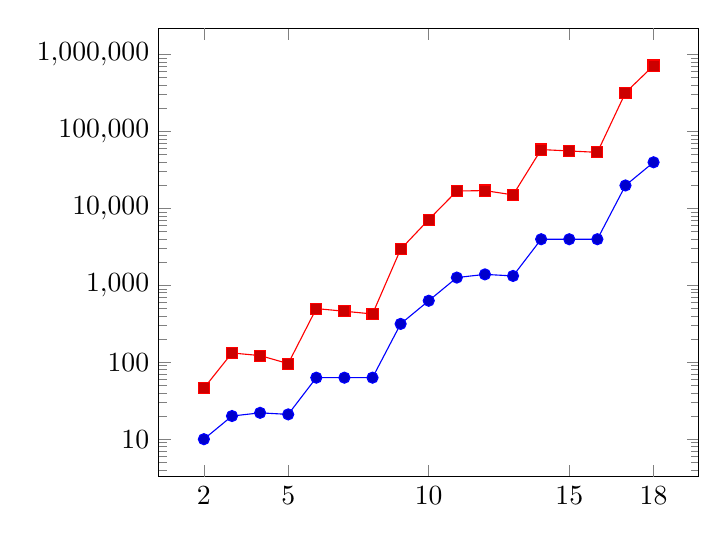
\begin{tikzpicture}
\begin{axis}[
    ymode=log,
    log ticks with fixed point,
    extra x ticks={2,18}
]
\addplot table {
	2 10
	3 20
	4 22
	5 21
	6 63
	7 63
	8 63
	9 315
	10 630
	11 1260
	12 1386
	13 1323
	14 3969
	15 3969
	16 3969
	17 19845
	18 39690 
};
\addplot table {
	2 46
	3 132
	4 122
	5 96
	6 498
	7 460
	8 424
	9 2939
	10 7138
	11 16796
	12 17014
	13 14952
	14 58086
	15 55692
	16 53424
	17 318717 	
	18 716814 
};
\end{axis}
\end{tikzpicture}
	\caption{Growth of the number of states (curve with round dots) and
	transitions (curve with square dots) while the growth of the number of modules
	in the centralized systems model}
	\label{fig:sync_growth}
\end{figure}


\subsection{Example of a failure verification}

For a demonstration of diagnosability verification with the developed tool
the instance of a hypothetical technological failure is taken (though it could
be a real case for the given system). A part of the material flow
description, given by a technologist is following.

Consider the P\&I diagram of the system  depicted in the Figure
\ref{fig:pi_diagram}. Volumes of the filter container and of the dust bucket are
chosen according to a speed the filter container fills up, the dust bucket
unloads and a speed of the material transportation by the both screw and
belt conveyers. When the filter container is filled, it takes two times to
load and unload the dust bucket. Due to physical limits of the process, the
filter conveyer can not be emptied with one load--unload cycle of the dust
bucket, neither the filter container can be full after two unload cycles.
An automaton model which may describe this technological process is depicted in
the Figure \ref{fig:system_failure02}.

The automaton reflects also possible failures (shown with the marked state of
the automaton).
If the filter container is empty just after one unload, this may be a symptom of the screw conveyer breakage,
destruction of the pipe or its connection to the valve. If the filter container
is full after three unload cycles, it may be a sign of low dust bucket
performance, pipes clogging, etc.

\begin{figure}[!ht]
	\centering
	\includegraphics[scale=0.7]{system_failure02.pdf}
	\caption{Model of a technological process failure}
	\label{fig:system_failure02}
\end{figure}

The failure automata model does not contain any observable events. Thus, the
model is not diagnosable locally. However, the model can be linked to the fork
level sensors $LT1$ and $LT3$ as with digital signals via cause-effect automata
(see description in the Appendix \ref{chap:automata_models}).

The diagnosability of the system was verified using the tool presented earlier.
The forward-propagation algorithm performed 356 compositions of the modules in
less then a second. During the failure propagation through the inference diagram
(see Figure \ref{fig:system_id}) six modules where updated while a little
complexity growth was observed. The verification has shown that in the diagnosis
of the failure two modules of the system participate, the sensors $LT1$ and
$LT3$. According to the approach of this work, these modules can be treated as
one virtual module. This virtual module can be used to build diagnoser for
online monitoring of the system, particularly for detection of the above
described failure.





% \section{Real example}


\chapter{Conclusions and future work}
\label{chap:conclusions}


\emph{``We are stuck with technology when what we really want is just stuff that
works'' -- Douglas Adams, The Salmon of Doubt}.

The main aim of this research was to bring the fascinating beauty of formal
mathematical approaches closer to everyday practices of industrial
development engineers in order to enhance the routine process of 
the automated systems creation.

As shown in this work, the major obstacle for application of formal methods in
the industrial systems development process seems to be a lack of appropriate
design techniques and tools. Despite the fact that the formal approaches are
generally quite mature, and in the field of Discrete Event Systems particularly,
there is still a room for improvements.
As a confirmation, one can observe that every-day design processes, decision
assistance, programming tools and languages are often outdated from the
perspective of what could be used nowadays.

To show the current situation in industry the Chapter
\ref{chap:problem_description} describes, with a help of an industrial plant
real example, what quantitative and qualitative methods are used nowadays,
besides the formal approaches, in order to achieve desired properties of
industrial systems.

A few goals were persuaded in this work. The first one is the modeling
approach for the manufacturing systems design. The effort has been taken in
the development of formal representations of widely used industrial components.
For this approach the framework of formal languages and automata has
been chosen. The choice is based on high availability of formal approaches
using this framework, which somehow confirms efficiency of these formalisms on
the one hand, and a relative simplicity of the mathematical notation and graphical
representation of automata models on the other hand, bearing in mind that the
results of the research should be understood by a wide community of industrial
engineers, with a little or no effort.

The automata design patterns, developed and validated during this research,
incorporate both nominal and faulty behaviours. This approach appeared to be
possible after decomposition of hardware components into small predefined
models. These models may efficiently abstract details of the
formal representation, and ``hide'' them from a designer of an
industrial system.
In order to increase the level of abstraction, thus enhancing usability and
reusability, the formal models are encapsulated into UML-like blocks of
Generalised Devices. This modeling process, as well as an essential mathematical
notation for discrete event systems in terms of languages and automata, and
diagnosability types are described in Chapter \ref{chap:framework}.

Use of the formal methods often corresponds with a problem of exponential
explosion which may make the a solution for the problem intractable. The
diagnosability analysis is not an exception. Approaches which rely on modular
nature of the complex system use a variety of notions and algorithmic techniques
in order to tackle the computational burden. This work has introduced a new
definition of diagnosability and a notion of virtual modules. It can be seen
as an algorithmic ``trick'' which combines the existing modules of the system
into new modules (which do not correspond to real components, and that
is why they are called ``virtual'') in a way that the system with the new
modularity is modular diagnosable. The theoretical part of this work is covered
in Chapter \ref{chap:theory}.

The final goal of the research was to focus on applicability of the developed
concepts. In order to validate the algorithms which verify diagnosability and
provide information for construction of virtual modules, a software tool has
been created. It is described in the Chapter \ref{chap:simulation}. There an
application of this tool for an instance of failure in the real
industrial process is demonstrated and compared with the centralized approach.

Concluding, modeling and theoretical approaches have been developed and then 
validated with a software tool, proving efficiency of the concepts.
Particularly, the performance advantage with respect to the centralized approach
is obvious. The advantages and disadvantages of the method with comparison to
other algorithmic techniques, even if they differ from the theoretical point of
view, has to be checked in the future.
Additional effort is also required for performance optimisations of the
developed software tool.


\appendix
\chapter{Automata models}
\label{chap:automata_models}

Here a set of automata models for some industrial entities is given. The
models are given both with no failure and failure behaviour. Failures are
reflected as events according to the event-based failure modeling approach and
as marked states for the state-based failure modeling approach. In the both
cases a marked state in a figure means that a fault occurred.  

\section{Digital Inputs/Outputs, Sensors, Motors, etc., and their connection}

\begin{figure}[th]
	\centering
	\includegraphics[scale=0.7]{lib_dido.pdf}
	\caption{General model of a digital input/output, relay, contactor, etc.}
	\label{fig:lib_dido}
\end{figure}


\begin{figure}[th]
	\centering
	\includegraphics[scale=0.7]{lib_dido_fail.pdf}
	\caption{Model of a digital input/output with failures}
	\label{fig:lib_dido_fail}
\end{figure}

The Figure \ref{fig:lib_dido} depicts a general model of a two-state component.
This model reflects behaviour of digital inputs/outputs, relays, contactors,
motors and other devices the behaviour of which can be equal to this
abstraction. The Figure \ref{fig:lib_dido_fail} depicts a faulty version of the
model. The faulty model reflects two failures: ``stuck low'' denoted as $f0$ and
``stuck high'' denoted as $f1$.

A consequent connection of two modules as the ones described above in a
cause-effect manner imposes constrain on the ``effect'' module. Assume that
there is two modules: $1$ -- ``cause'' (e.g. a contactor) and $2$ -- ``effect''
(e.g a motor). The model of the constrain and the result of composition of the
entire system (two components and their constrain) is depicted in Figure
\ref{fig:lib_2do}. If the module $1$ has failures modeled as shown in Figure
\ref{fig:lib_dido_fail}, then the entire system looks as in Figure
\ref{fig:lib_2do_fail}.

A model of the same failure can be presented using the state-based
failure approach. In this case no fault events are used. Since the model of
a digital signal defines its full language, the model of the constrain has to be
exploited instead, as shown in the Figure \ref{fig:lib_2do_fail2}. The resulting
composition has lower complexity. It has a positive effect for the
computation burden during verification of complex systems, since almost any
industrial system includes many digital inputs, outputs and other similar
components. However, it is arguable what model should include the failure of the
component, the model of the component itself or models of constrains.


\begin{figure}[!th]
	\centering
	\includegraphics[scale=0.7]{lib_do2do.pdf}
	\includegraphics[scale=0.7]{lib_2do.pdf}
	\caption{The constrain model (left) for two consequent two-state components,
	and the result of the composition of the entire system (right)}
	\label{fig:lib_2do}
\end{figure}

\begin{figure}[!th]
	\centering
	\includegraphics[scale=0.7]{lib_2do_fail.pdf}
	\caption{Fault model of two consequent digital two-state modules. The
	first module has failures}
	\label{fig:lib_2do_fail}
\end{figure}


\begin{figure}[!th]
	\centering
	\includegraphics[scale=0.7]{lib_do2do_fail.pdf}
	\includegraphics[scale=0.7]{lib_2do_fail2.pdf}
	\caption{The cause-effect fault automaton model (left), and the resulting
	composition of two components (right)}
	\label{fig:lib_2do_fail2}
\end{figure}

\begin{figure}[!th]
	\centering
	\includegraphics[scale=0.7]{lib_do2do_fail3.pdf}
	\includegraphics[scale=0.7]{lib_2do_fail3.pdf}
	\caption{The model of the constrain (left) and the composition result (right).
	Failures are in the second (i.e. ``effect") module}
	\label{fig:lib_2do_fail3}
\end{figure}

A consequent connection of two modules: $1$ -- ``cause'' (e.g. a contactor) and
$2$ -- ``effect'' (e.g. a motor), where the second module has failures is
depicted in Figure \ref{fig:lib_2do_fail3}. Here the failures are modeled using
state-based failure approach.


\section{Valve}

The most known physical model of a valve is depicted in the Figure
\ref{fig:lib_valve}.
The model reflects a wide variety of valves, e.g. gate valves, butterfly valves,
ball valves, etc. In general, five states if this type of equipment can be
distinguished: two boundary states (closed and open), two movement states
(opening, closing) and stop in an intermediate position.

The ``stop'' position of the gate valve model can be marked as faulty,
since gate valves must usually stay either closed or open.

\begin{figure}[!th]
	\centering
	\includegraphics[scale=0.7]{lib_valve.pdf}
	\caption{Automaton model of a valve}
	\label{fig:lib_valve}
\end{figure}


\subsection{Valve with sensors}

Figure \ref{fig:lib_valve2sensor1} shows the model of a sensor $1$ built
according to the model of two-state components described before, and a constrain
model which assumes that the sensor observes ``closed'' state of the valve.
From the perspective of the sensor the valve can be either closed or not. In
another words, the valve is seen as a two-state component. Thus, the constrain
automaton similar to the one shown in the Figure \ref{fig:lib_2do} can be used.

\begin{figure}[th]
	\centering
	\includegraphics[scale=0.7]{lib_sensor1.pdf}
	\includegraphics[scale=0.7]{lib_valve2sensor1.pdf}	
	\caption{Automata of a sensor and a constrain model for the sensor--valve
	relationship}
	\label{fig:lib_valve2sensor1}
\end{figure}

Let the valve to have two sensor: one for the closed state and another
one for the open state. An inference diagram of such system is shown in the
Figure \ref{fig:lib_id_valve+2sensors}. It reflects the coupling of all the
corresponding models, e.g. valve, two sensors ($S1$, $S2$) and their
constrains. The result of the composition of is depicted in the Figure
\ref{fig:lib_valve+2sensors}. The purpose of the figure is to show the level of
complexity of such simple system.

A fault model of the valve's sensors is equal to the one depicted in the Figure
\ref{fig:lib_dido_fail}.

\begin{figure}[!th]
	\centering
	\includegraphics[scale=0.7]{lib_id_valve+2sensors.pdf}
	\caption{Inference diagram of a valve with two sensors}
	\label{fig:lib_id_valve+2sensors}
\end{figure}

 
\begin{figure}[th]
	\centering
	\includegraphics[scale=0.7]{lib_valve+2sensors.pdf}
	\caption{Automaton of a valve with two sensors (open and closed)}
	\label{fig:lib_valve+2sensors}
\end{figure}


\subsection{Valve with actuator} 

Automaton model of a double actuation device for a valve is depicted in the
Figure \ref{fig:lib_act} (think of an bidirectional motor). Actually, it has two
actuating parts, denoted in the figure by  prefixes $a$ and $b$. Part $a$ is responsible for the ``opening''
movement, part $b$ is responsible for the ``closing'' movement. Each actuating
part is equal to the two-state digital component model, presented before.
In the composition of these two components a consequent execution of events
$a_hi$ and $b_hi$ is forbidden, i.e. it is necessary that $a\_hi \Rightarrow
b\_lo$ and $b\_hi \Rightarrow a\_lo$.

\begin{figure}[!ht]
	\centering
	\includegraphics[scale=0.7]{lib_act.pdf}
	\caption{Automaton of a valve actuator}
	\label{fig:lib_act}
\end{figure}


\begin{figure}[!ht]
	\centering  
	\includegraphics[scale=0.7]{lib_valve2actuator_a.pdf}
	\includegraphics[scale=0.7]{lib_valve2actuator_b.pdf}
	\caption{Automata of the valve actuator constrains}
	\label{fig:lib_valve2actuator_a}
\end{figure}

The actuation devices are coupled with the physical valve model through a 
constrain automaton, similar to described above. The constrain automata for
the valve are shown in the Figure \ref{fig:lib_valve2actuator_a}. 
The result of the composition of the valve, actuator and constrains is depicted
in the Figure \ref{fig:lib_valve+actuator}. Marked states are correspond to the
``stop'' state of the valve, which may be considered as a fault for a
gate valve.

\begin{figure}[!ht]
	\centering
	\includegraphics[scale=0.7]{lib_valve+actuator.pdf}
	\caption{Automaton of a valve with the actuator}
	\label{fig:lib_valve+actuator}
\end{figure}


\subsection{Valve with sensors and actuator}

Automaton which represents the complete model, i.e. the composition of the valve
with two sensors and the actuator has 63 states and 424 transitions. A
corresponding inference diagram is shown in the Figure
\ref{fig:lib_valve+2sensors+actuator}. Meaning of the nodes names is explained
in the table below.

\begin{figure}[!ht]
	\centering
	\includegraphics[scale=0.7]{lib_valve+2sensors+actuator.pdf}
	\caption{Inference diagram of a valve with two sensor and an actuator (see
	Table \ref{tbl:id_valve+2sensors+actuator} for the nodes names description)}
	\label{fig:lib_valve+2sensors+actuator}
\end{figure}

\begin{table}[!ht]
\caption{Nodes labels of the inference diagram of the valve, sensors and
actuator}
\centering
	\begin{tabular}{l l}
	\\	
	Node label & Description\\
	\hline
	v1 & Valve\\
	v1so & Sensor ``Open"\\
	v1sc & Sensor ``Closed"\\
	v1-v1so & Constrain of the valve to the sensor ``Open"\\
	v1-v1sc & Constrain of the valve to the sensor ``Closed"\\
	a & Actuator\\
	a\_a-v1 & Constrain of the valve to the actuator's part ``Opening"\\
	a\_b-v1 & Constrain of the valve to the actuator's part ``Closing"
	\end{tabular}
	\label{tbl:id_valve+2sensors+actuator}
\end{table}



\clearpage
\newpage

% \include{biblio}

\bibliography{References}
\bibliographystyle{plain}


\end{document}
